\documentclass[11pt]{article}
\usepackage[textwidth=18.0cm, textheight=23.0cm, top=2.0cm]{geometry}
\usepackage{pst-all}
\usepackage{amssymb}
\usepackage{tikz}
\usepackage{underscore}\begin{document}
\pagestyle{empty}


ClassName: \underline{\textbf{Class_03.2bp-44}}
\par
BinSize: \underline{\textbf{40 × 40}}
\par
ReduceSize: \underline{\textbf{40 × 40}}
\par
TypeNum: \underline{\textbf{98}}
\par
Num: \underline{\textbf{100}}
\par
OutS: \underline{\textbf{35200}}
\par
InS: \underline{\textbf{32327}}
\par
Rate: \underline{\textbf{0.918}}
\par
UB: \underline{\textbf{22}}
\par
LB0: \underline{\textbf{22}}
\par
LB: \underline{\textbf{22}}
\par
LBWithCut: \underline{\textbf{22}}
\par
NodeCut: \underline{\textbf{0}}
\par
ExtendedNodeCnt: \underline{\textbf{1}}
\par
GenNodeCnt: \underline{\textbf{1}}
\par
PrimalNode: \underline{\textbf{0}}
\par
ColumnCount: \underline{\textbf{22}}
\par
TotalCutCount: \underline{\textbf{0}}
\par
RootCutCount: \underline{\textbf{0}}
\par
LPSolverCnt: \underline{\textbf{1}}
\par
PricingSolverCnt: \underline{\textbf{0}}
\par
BranchAndBoundNum: \underline{\textbf{1}}
\par
isOpt: \underline{\textbf{true}}
\par
TimeOnInitSolution: \underline{\textbf{0.750 s}}
\par
TimeOnPrimal: \underline{\textbf{0.000 s}}
\par
TimeOnPricing: \underline{\textbf{0.000 s}}
\par
TimeOnRmp: \underline{\textbf{0.078 s}}
\par
TotalTime: \underline{\textbf{0.906 s}}
\par
\newpage


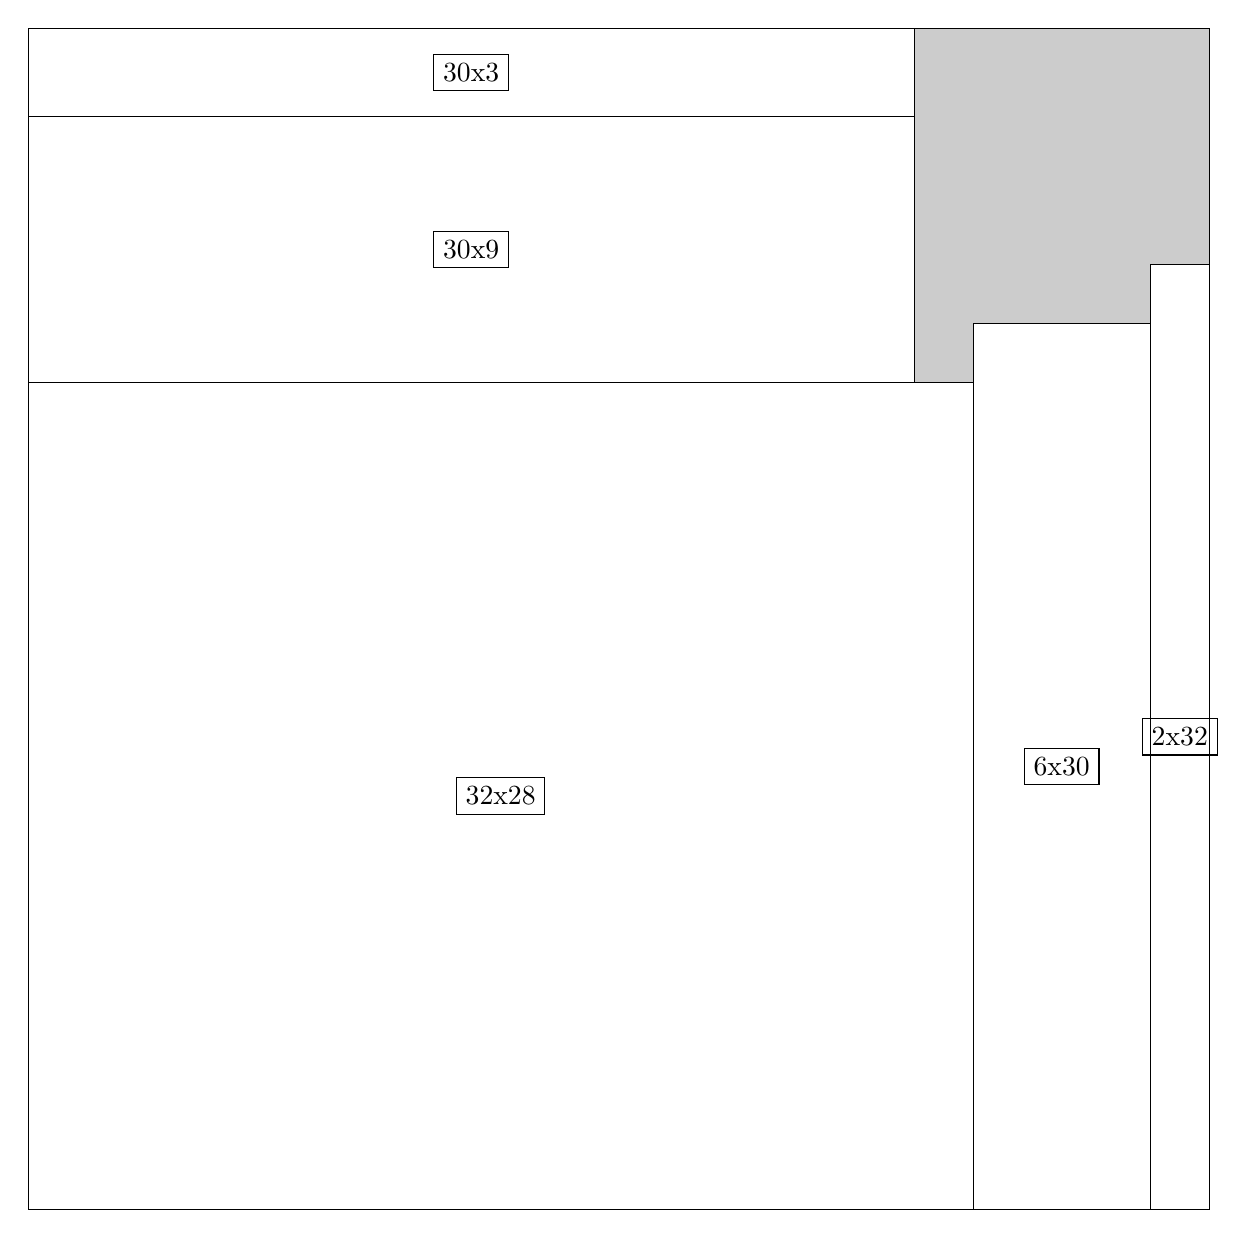
\begin{tikzpicture}[shorten >=1pt,scale=1.0,every node/.style={scale=1.0},->]
\tikzstyle{vertex}=[circle,fill=black!25,minimum size=14pt,inner sep=0pt]
\filldraw[fill=gray!40!white, draw=black] (0,0) rectangle (15.0,15.0);
\foreach \name/\x/\y/\w/\h in {32x28/0.0/0.0/12.0/10.5,30x9/0.0/10.5/11.25/3.375,6x30/12.0/0.0/2.25/11.25,30x3/0.0/13.875/11.25/1.125,2x32/14.25/0.0/0.75/12.0}
\filldraw[fill=white!40!white, draw=black] (\x,\y) rectangle node[draw] (\name) {\name} ++(\w,\h);
\end{tikzpicture}


w =32 , h =28 , x =0 , y =0 , v =896
\par
w =30 , h =9 , x =0 , y =28 , v =270
\par
w =6 , h =30 , x =32 , y =0 , v =180
\par
w =30 , h =3 , x =0 , y =37 , v =90
\par
w =2 , h =32 , x =38 , y =0 , v =64
\par
\newpage


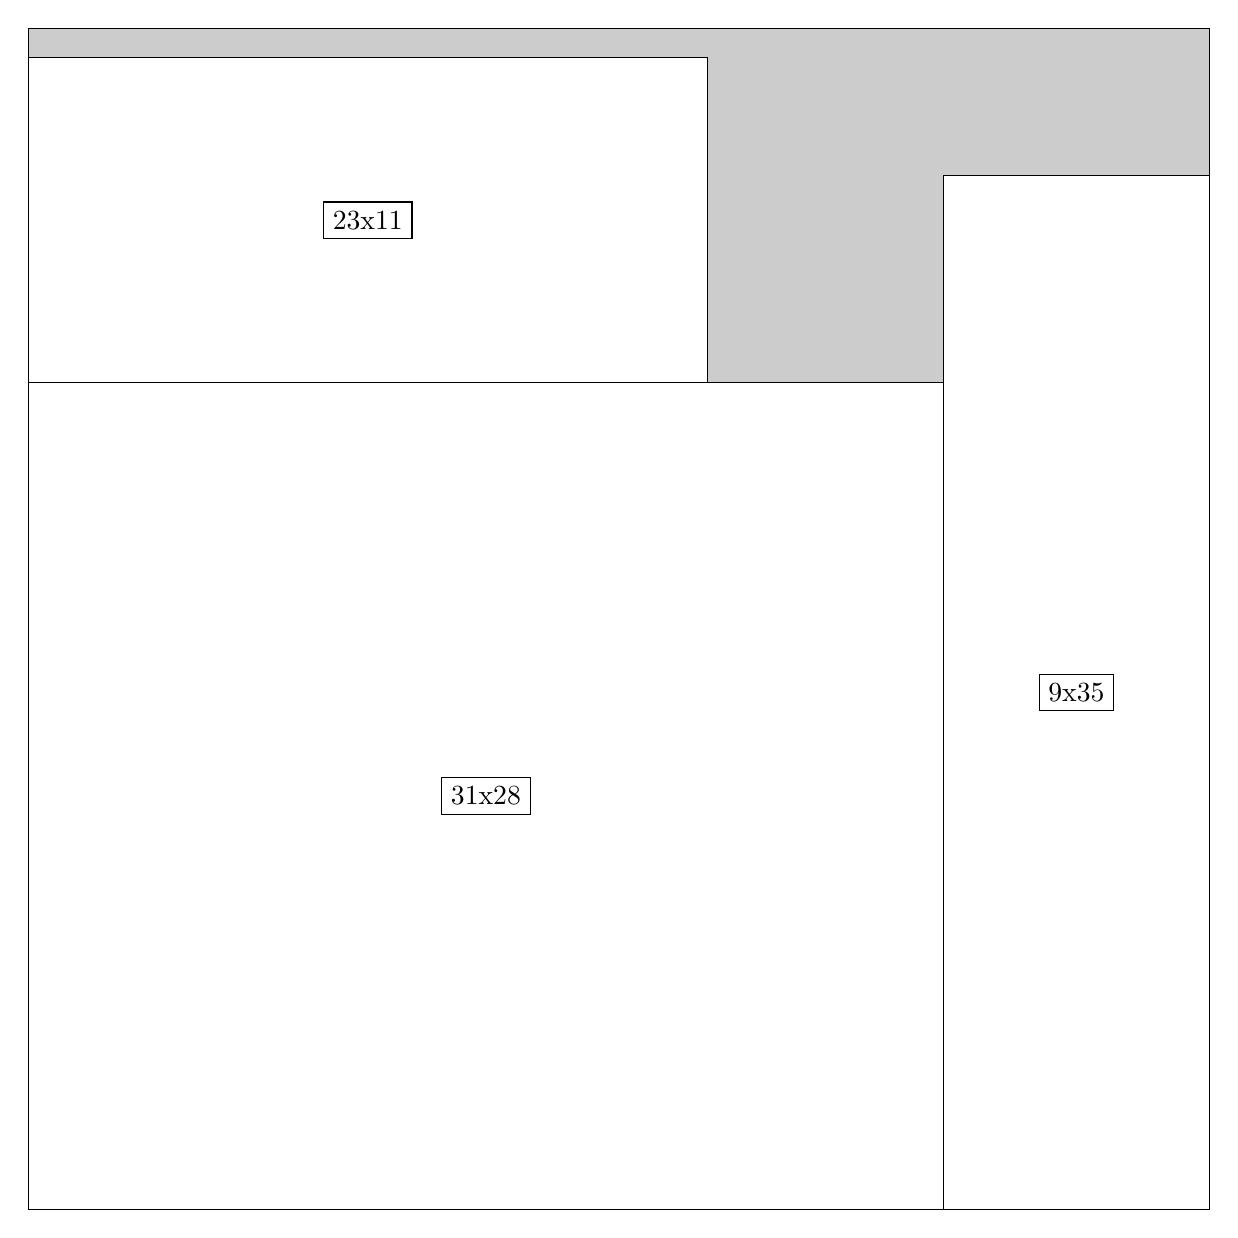
\begin{tikzpicture}[shorten >=1pt,scale=1.0,every node/.style={scale=1.0},->]
\tikzstyle{vertex}=[circle,fill=black!25,minimum size=14pt,inner sep=0pt]
\filldraw[fill=gray!40!white, draw=black] (0,0) rectangle (15.0,15.0);
\foreach \name/\x/\y/\w/\h in {31x28/0.0/0.0/11.625/10.5,9x35/11.625/0.0/3.375/13.125,23x11/0.0/10.5/8.625/4.125}
\filldraw[fill=white!40!white, draw=black] (\x,\y) rectangle node[draw] (\name) {\name} ++(\w,\h);
\end{tikzpicture}


w =31 , h =28 , x =0 , y =0 , v =868
\par
w =9 , h =35 , x =31 , y =0 , v =315
\par
w =23 , h =11 , x =0 , y =28 , v =253
\par
\newpage


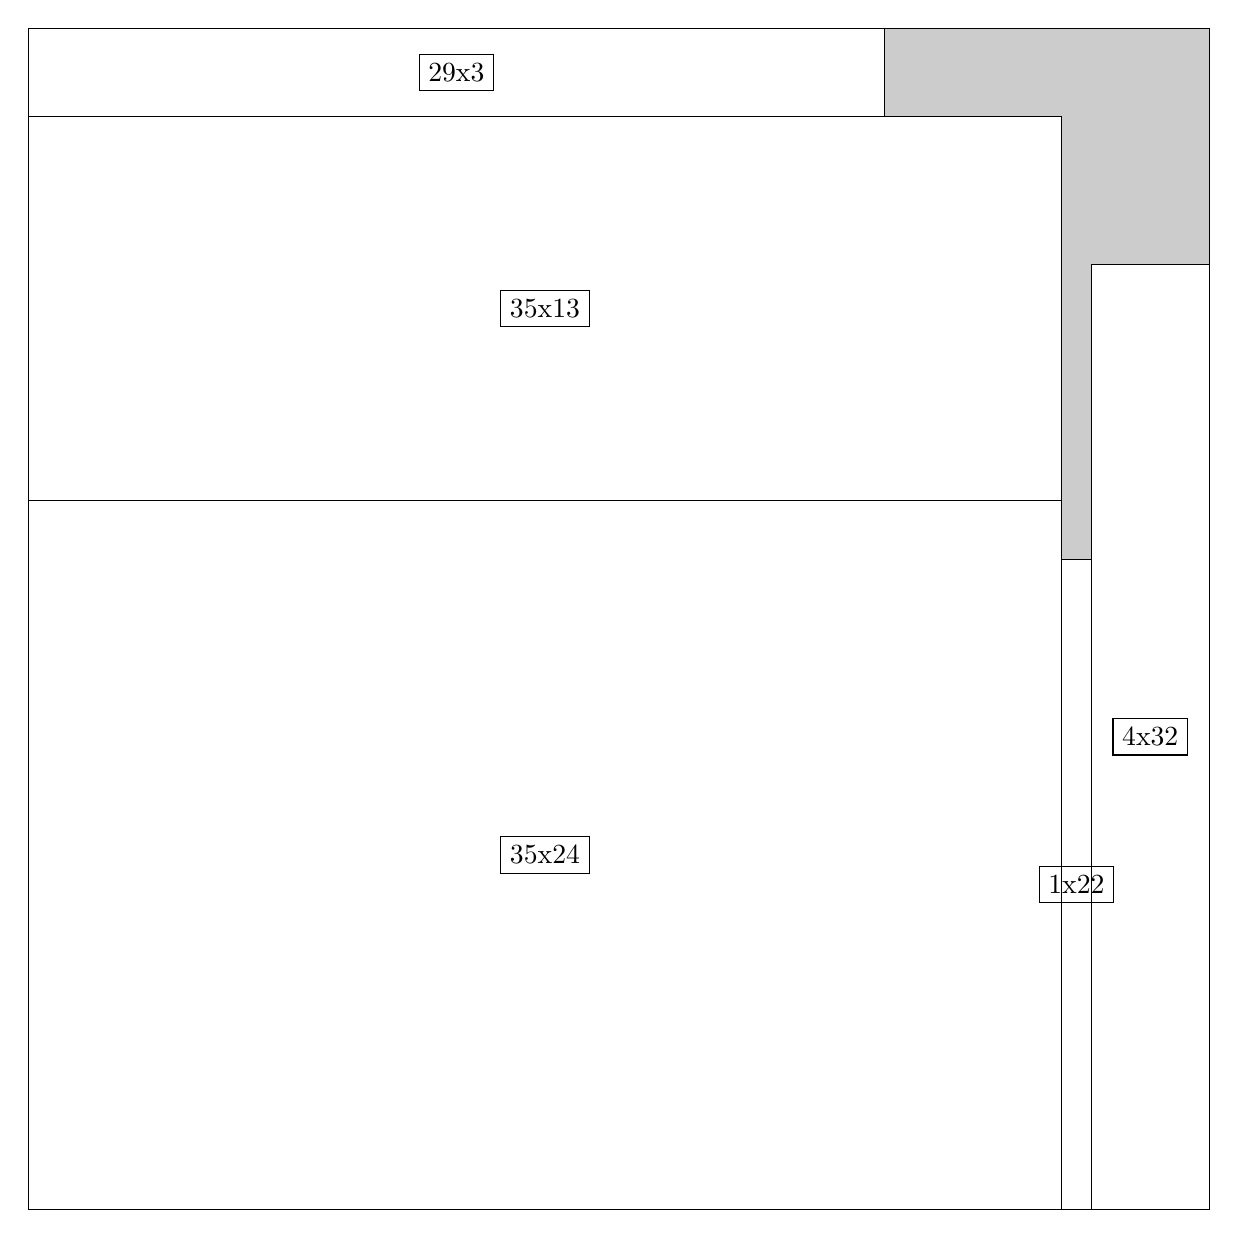
\begin{tikzpicture}[shorten >=1pt,scale=1.0,every node/.style={scale=1.0},->]
\tikzstyle{vertex}=[circle,fill=black!25,minimum size=14pt,inner sep=0pt]
\filldraw[fill=gray!40!white, draw=black] (0,0) rectangle (15.0,15.0);
\foreach \name/\x/\y/\w/\h in {35x24/0.0/0.0/13.125/9.0,35x13/0.0/9.0/13.125/4.875,4x32/13.5/0.0/1.5/12.0,29x3/0.0/13.875/10.875/1.125,1x22/13.125/0.0/0.375/8.25}
\filldraw[fill=white!40!white, draw=black] (\x,\y) rectangle node[draw] (\name) {\name} ++(\w,\h);
\end{tikzpicture}


w =35 , h =24 , x =0 , y =0 , v =840
\par
w =35 , h =13 , x =0 , y =24 , v =455
\par
w =4 , h =32 , x =36 , y =0 , v =128
\par
w =29 , h =3 , x =0 , y =37 , v =87
\par
w =1 , h =22 , x =35 , y =0 , v =22
\par
\newpage


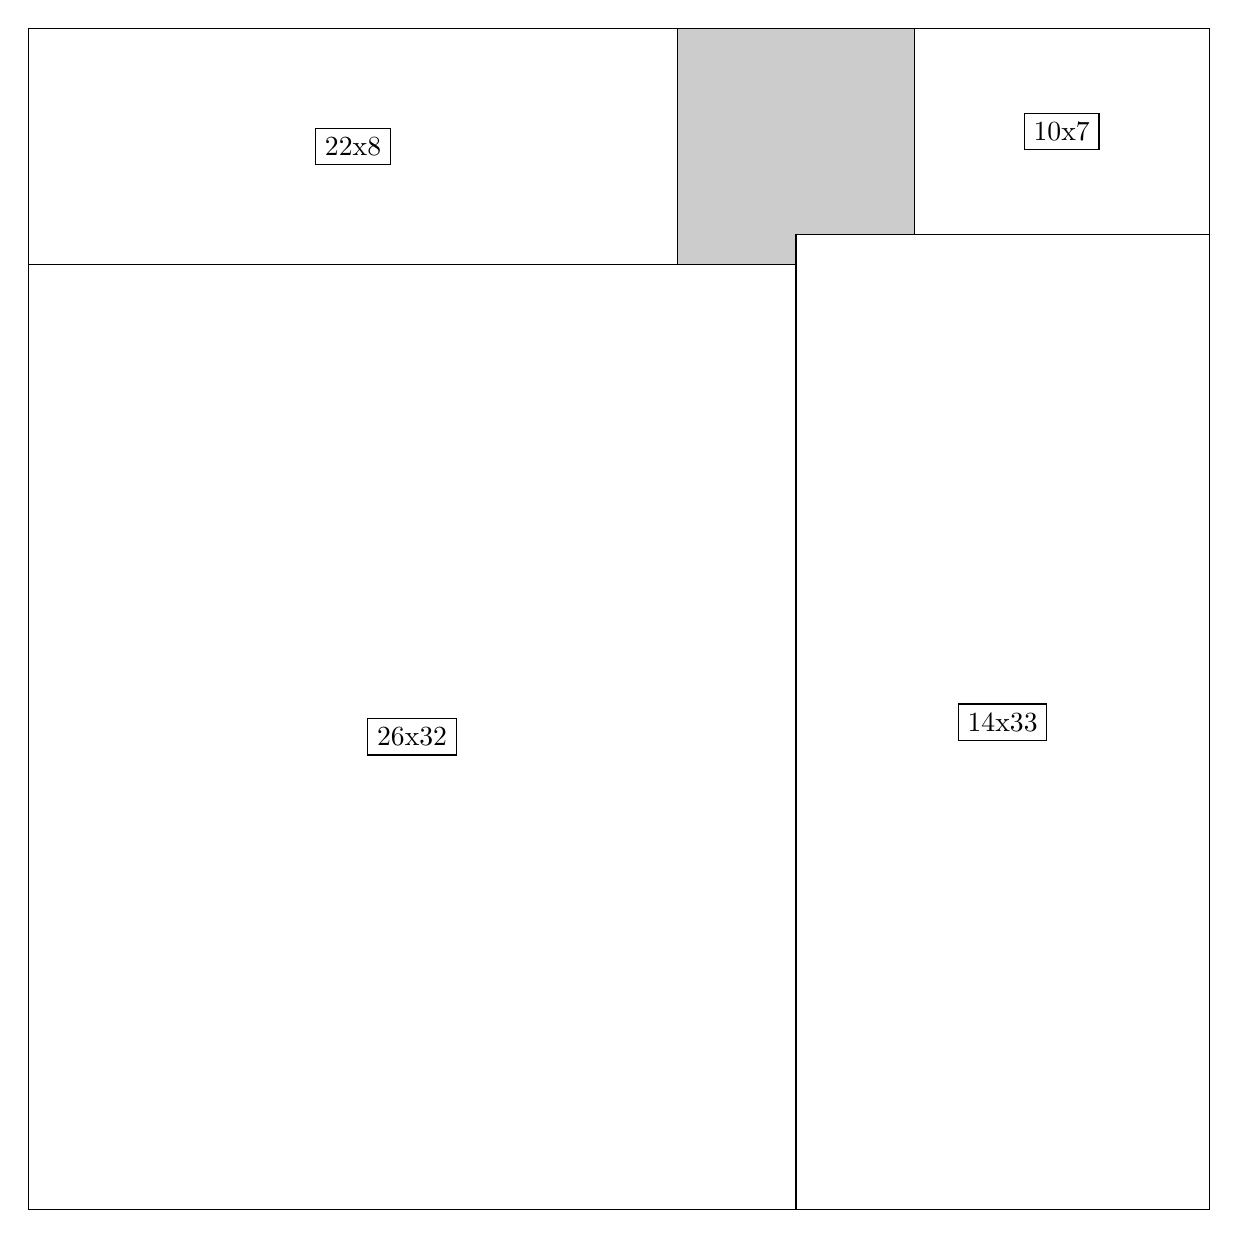
\begin{tikzpicture}[shorten >=1pt,scale=1.0,every node/.style={scale=1.0},->]
\tikzstyle{vertex}=[circle,fill=black!25,minimum size=14pt,inner sep=0pt]
\filldraw[fill=gray!40!white, draw=black] (0,0) rectangle (15.0,15.0);
\foreach \name/\x/\y/\w/\h in {26x32/0.0/0.0/9.75/12.0,14x33/9.75/0.0/5.25/12.375,22x8/0.0/12.0/8.25/3.0,10x7/11.25/12.375/3.75/2.625}
\filldraw[fill=white!40!white, draw=black] (\x,\y) rectangle node[draw] (\name) {\name} ++(\w,\h);
\end{tikzpicture}


w =26 , h =32 , x =0 , y =0 , v =832
\par
w =14 , h =33 , x =26 , y =0 , v =462
\par
w =22 , h =8 , x =0 , y =32 , v =176
\par
w =10 , h =7 , x =30 , y =33 , v =70
\par
\newpage


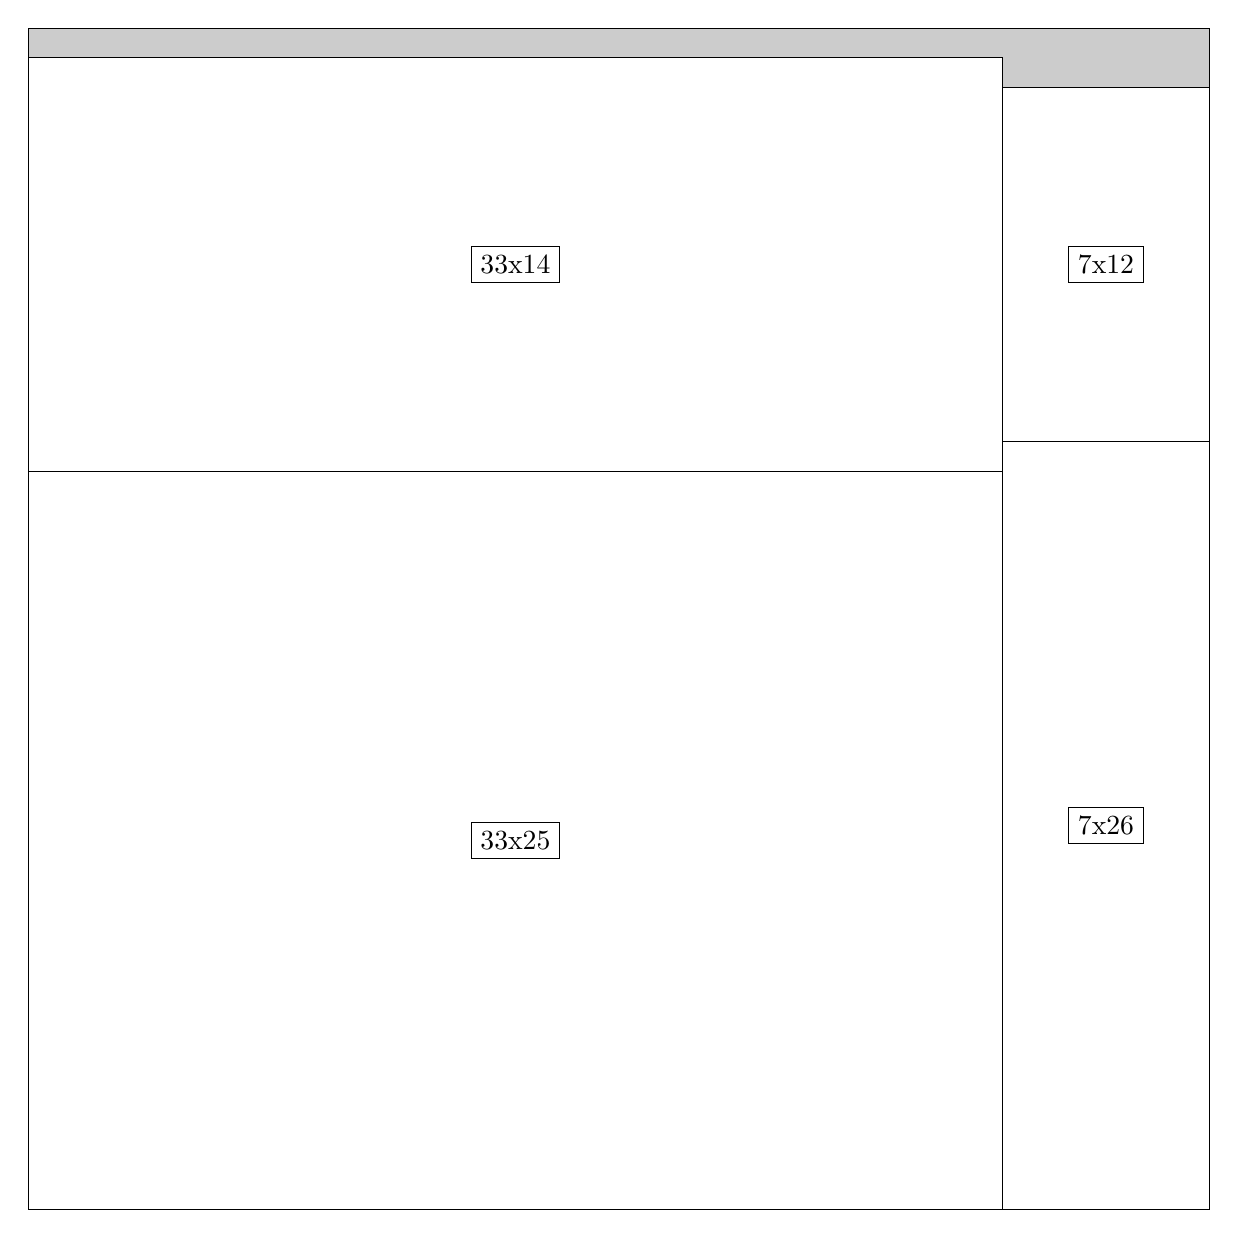
\begin{tikzpicture}[shorten >=1pt,scale=1.0,every node/.style={scale=1.0},->]
\tikzstyle{vertex}=[circle,fill=black!25,minimum size=14pt,inner sep=0pt]
\filldraw[fill=gray!40!white, draw=black] (0,0) rectangle (15.0,15.0);
\foreach \name/\x/\y/\w/\h in {33x25/0.0/0.0/12.375/9.375,33x14/0.0/9.375/12.375/5.25,7x26/12.375/0.0/2.625/9.75,7x12/12.375/9.75/2.625/4.5}
\filldraw[fill=white!40!white, draw=black] (\x,\y) rectangle node[draw] (\name) {\name} ++(\w,\h);
\end{tikzpicture}


w =33 , h =25 , x =0 , y =0 , v =825
\par
w =33 , h =14 , x =0 , y =25 , v =462
\par
w =7 , h =26 , x =33 , y =0 , v =182
\par
w =7 , h =12 , x =33 , y =26 , v =84
\par
\newpage


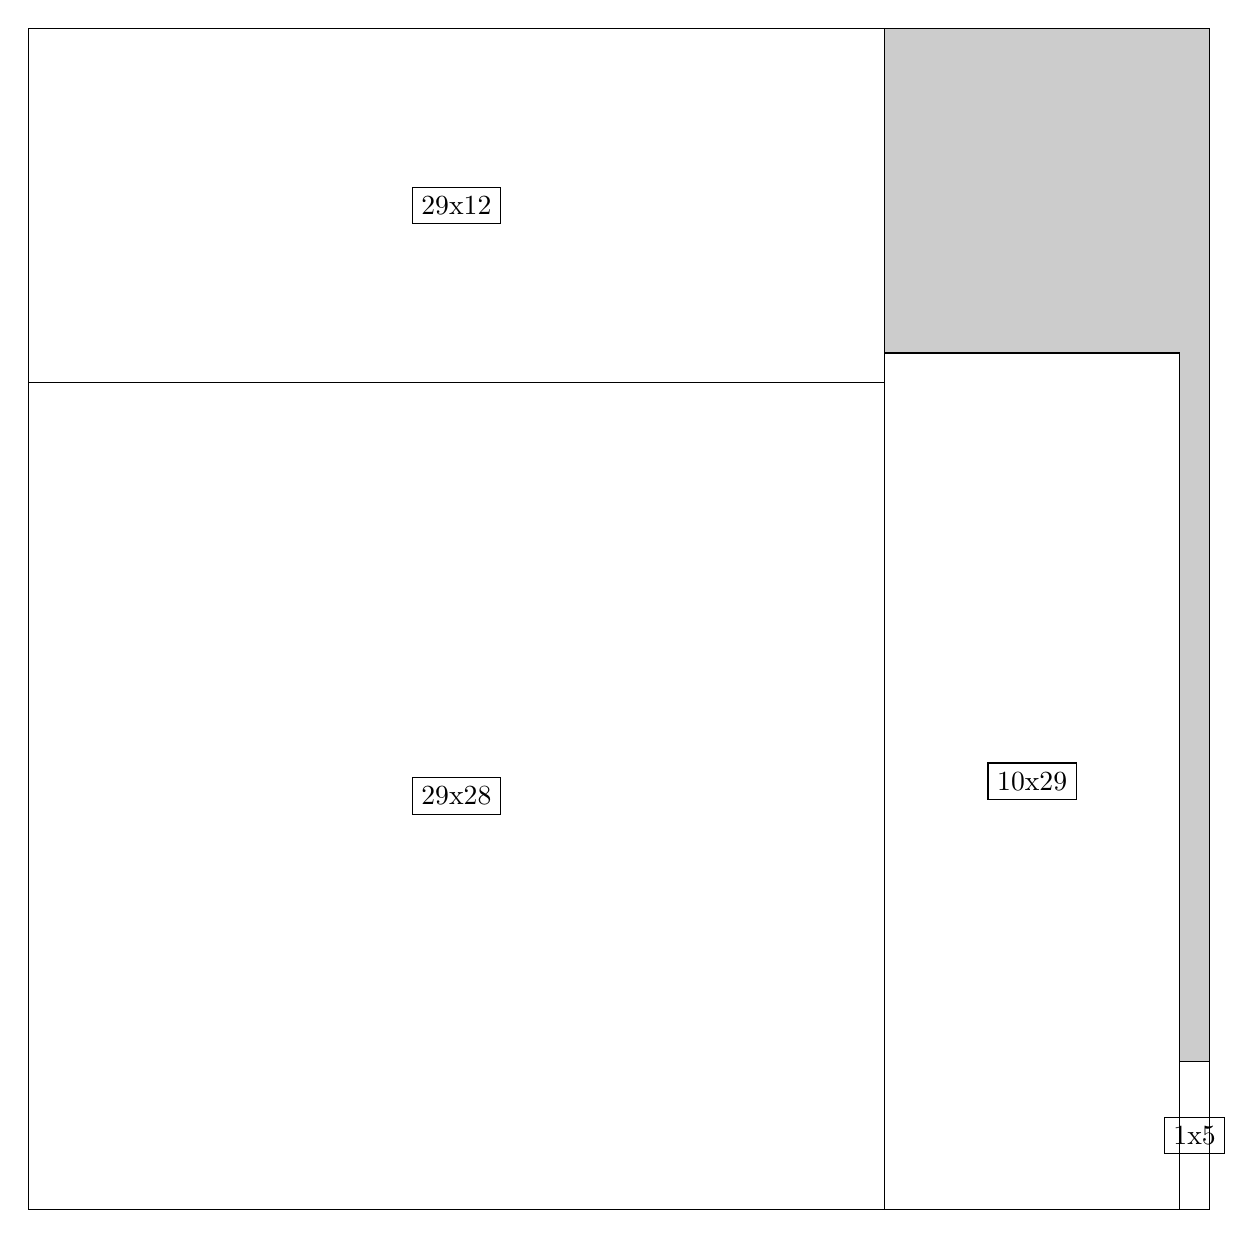
\begin{tikzpicture}[shorten >=1pt,scale=1.0,every node/.style={scale=1.0},->]
\tikzstyle{vertex}=[circle,fill=black!25,minimum size=14pt,inner sep=0pt]
\filldraw[fill=gray!40!white, draw=black] (0,0) rectangle (15.0,15.0);
\foreach \name/\x/\y/\w/\h in {29x28/0.0/0.0/10.875/10.5,29x12/0.0/10.5/10.875/4.5,10x29/10.875/0.0/3.75/10.875,1x5/14.625/0.0/0.375/1.875}
\filldraw[fill=white!40!white, draw=black] (\x,\y) rectangle node[draw] (\name) {\name} ++(\w,\h);
\end{tikzpicture}


w =29 , h =28 , x =0 , y =0 , v =812
\par
w =29 , h =12 , x =0 , y =28 , v =348
\par
w =10 , h =29 , x =29 , y =0 , v =290
\par
w =1 , h =5 , x =39 , y =0 , v =5
\par
\newpage


\begin{tikzpicture}[shorten >=1pt,scale=1.0,every node/.style={scale=1.0},->]
\tikzstyle{vertex}=[circle,fill=black!25,minimum size=14pt,inner sep=0pt]
\filldraw[fill=gray!40!white, draw=black] (0,0) rectangle (15.0,15.0);
\foreach \name/\x/\y/\w/\h in {27x30/0.0/0.0/10.125/11.25,13x35/10.125/0.0/4.875/13.125,27x7/0.0/11.25/10.125/2.625,27x3/0.0/13.875/10.125/1.125,10x5/10.125/13.125/3.75/1.875}
\filldraw[fill=white!40!white, draw=black] (\x,\y) rectangle node[draw] (\name) {\name} ++(\w,\h);
\end{tikzpicture}


w =27 , h =30 , x =0 , y =0 , v =810
\par
w =13 , h =35 , x =27 , y =0 , v =455
\par
w =27 , h =7 , x =0 , y =30 , v =189
\par
w =27 , h =3 , x =0 , y =37 , v =81
\par
w =10 , h =5 , x =27 , y =35 , v =50
\par
\newpage


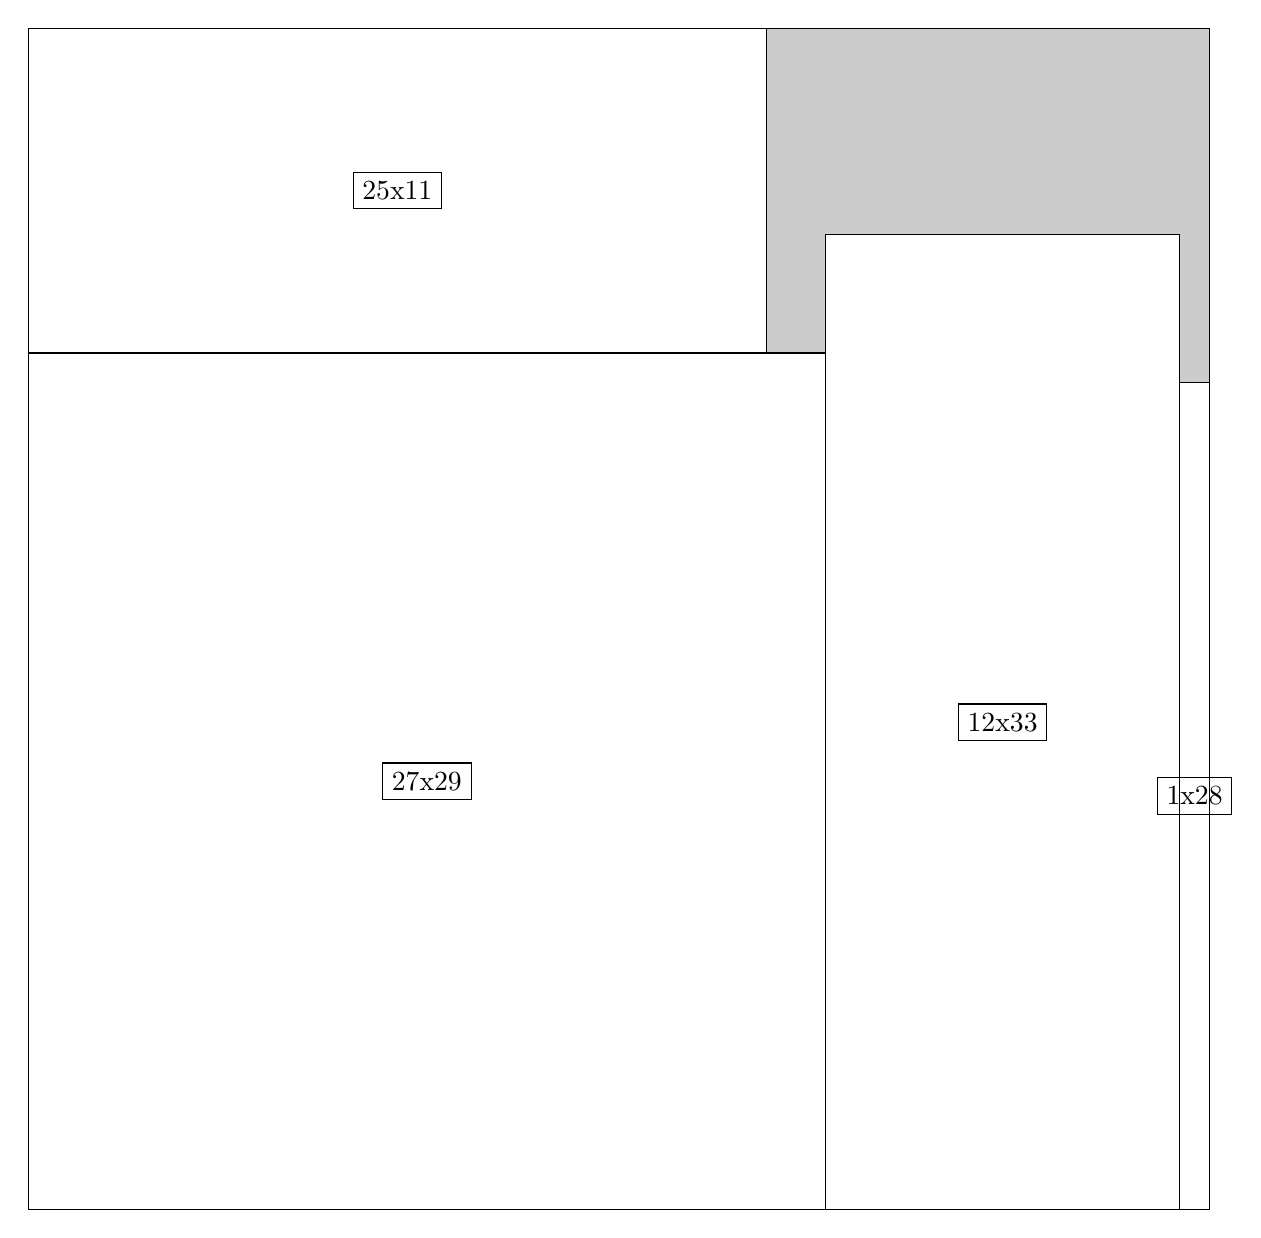
\begin{tikzpicture}[shorten >=1pt,scale=1.0,every node/.style={scale=1.0},->]
\tikzstyle{vertex}=[circle,fill=black!25,minimum size=14pt,inner sep=0pt]
\filldraw[fill=gray!40!white, draw=black] (0,0) rectangle (15.0,15.0);
\foreach \name/\x/\y/\w/\h in {27x29/0.0/0.0/10.125/10.875,12x33/10.125/0.0/4.5/12.375,25x11/0.0/10.875/9.375/4.125,1x28/14.625/0.0/0.375/10.5}
\filldraw[fill=white!40!white, draw=black] (\x,\y) rectangle node[draw] (\name) {\name} ++(\w,\h);
\end{tikzpicture}


w =27 , h =29 , x =0 , y =0 , v =783
\par
w =12 , h =33 , x =27 , y =0 , v =396
\par
w =25 , h =11 , x =0 , y =29 , v =275
\par
w =1 , h =28 , x =39 , y =0 , v =28
\par
\newpage


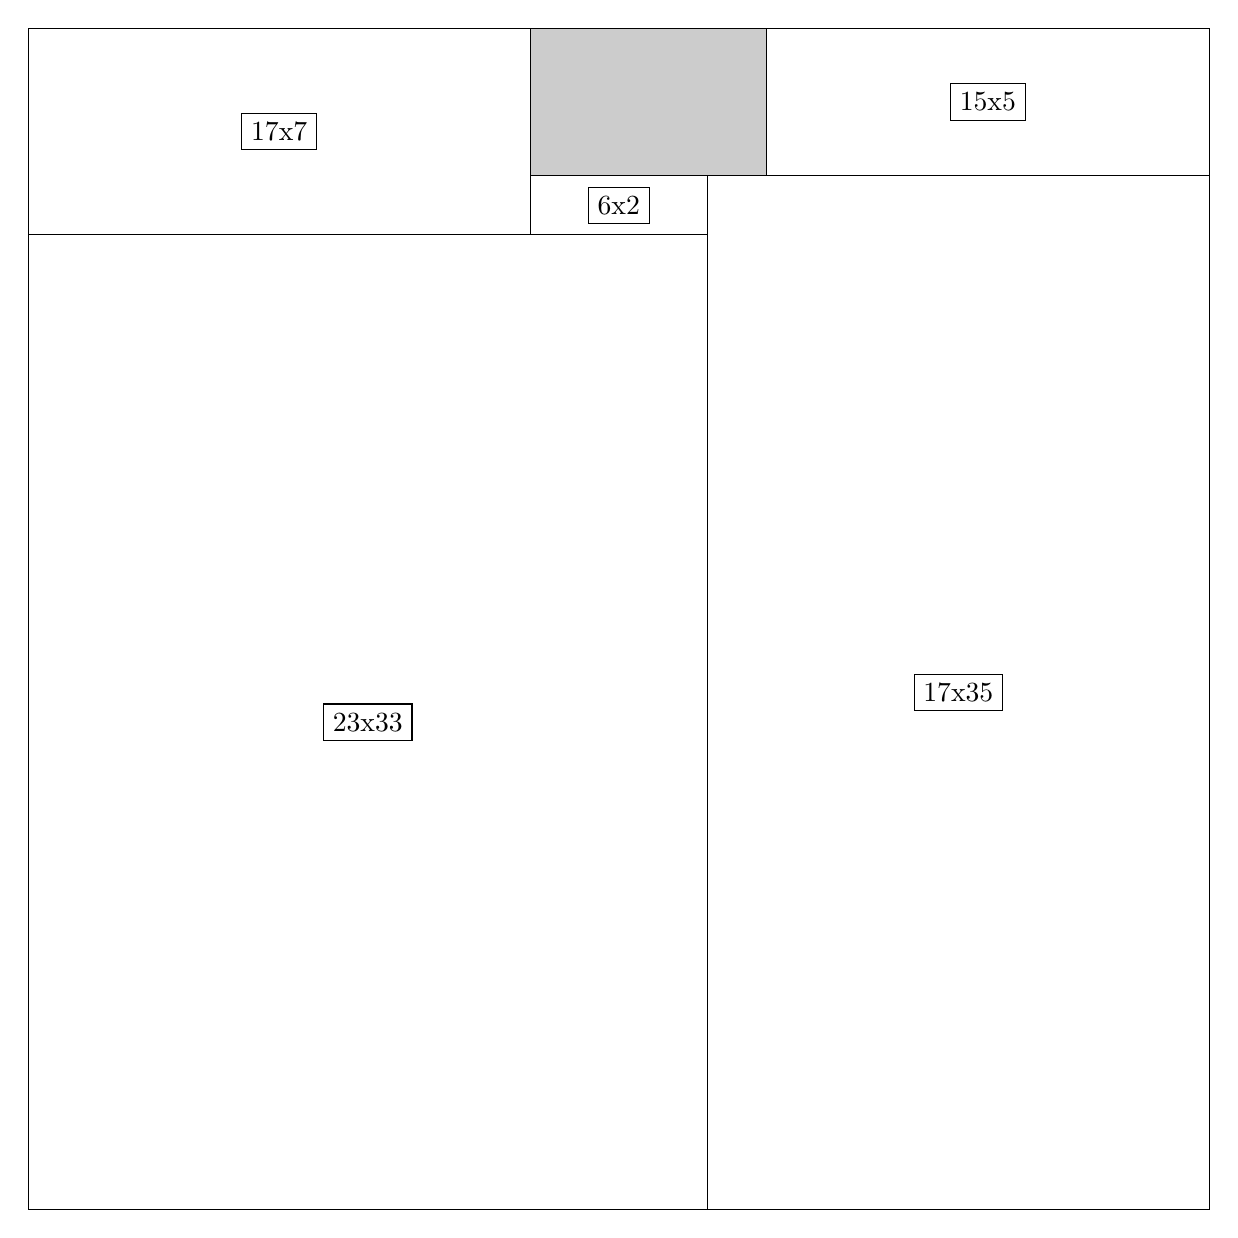
\begin{tikzpicture}[shorten >=1pt,scale=1.0,every node/.style={scale=1.0},->]
\tikzstyle{vertex}=[circle,fill=black!25,minimum size=14pt,inner sep=0pt]
\filldraw[fill=gray!40!white, draw=black] (0,0) rectangle (15.0,15.0);
\foreach \name/\x/\y/\w/\h in {23x33/0.0/0.0/8.625/12.375,17x35/8.625/0.0/6.375/13.125,17x7/0.0/12.375/6.375/2.625,15x5/9.375/13.125/5.625/1.875,6x2/6.375/12.375/2.25/0.75}
\filldraw[fill=white!40!white, draw=black] (\x,\y) rectangle node[draw] (\name) {\name} ++(\w,\h);
\end{tikzpicture}


w =23 , h =33 , x =0 , y =0 , v =759
\par
w =17 , h =35 , x =23 , y =0 , v =595
\par
w =17 , h =7 , x =0 , y =33 , v =119
\par
w =15 , h =5 , x =25 , y =35 , v =75
\par
w =6 , h =2 , x =17 , y =33 , v =12
\par
\newpage


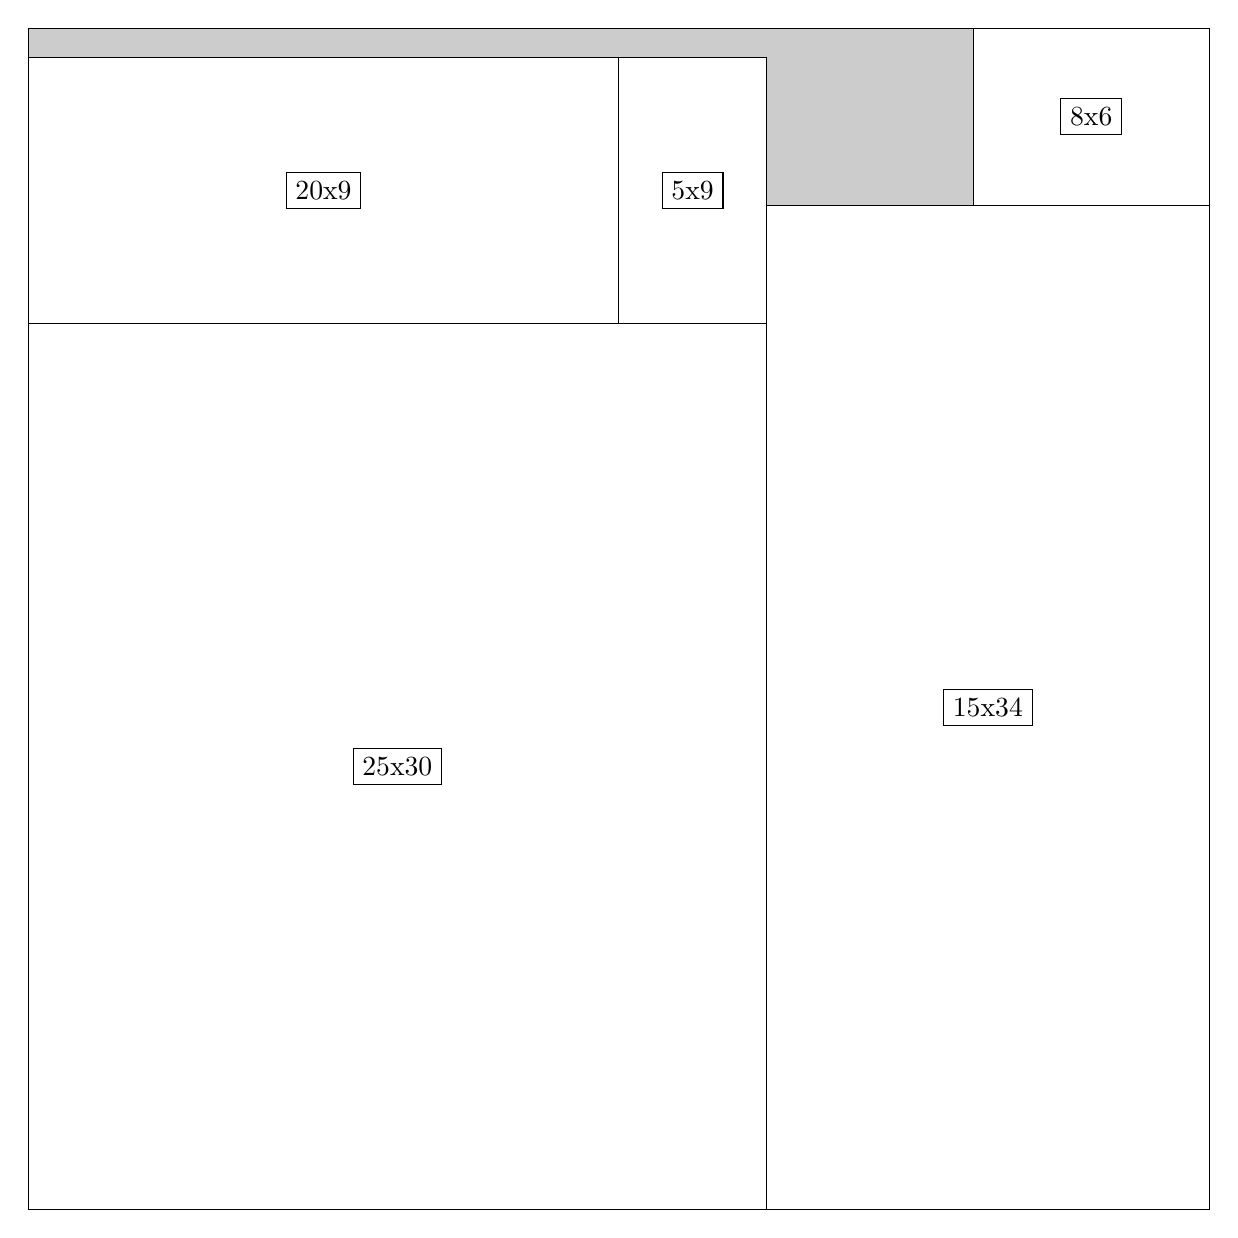
\begin{tikzpicture}[shorten >=1pt,scale=1.0,every node/.style={scale=1.0},->]
\tikzstyle{vertex}=[circle,fill=black!25,minimum size=14pt,inner sep=0pt]
\filldraw[fill=gray!40!white, draw=black] (0,0) rectangle (15.0,15.0);
\foreach \name/\x/\y/\w/\h in {25x30/0.0/0.0/9.375/11.25,15x34/9.375/0.0/5.625/12.75,20x9/0.0/11.25/7.5/3.375,8x6/12.0/12.75/3.0/2.25,5x9/7.5/11.25/1.875/3.375}
\filldraw[fill=white!40!white, draw=black] (\x,\y) rectangle node[draw] (\name) {\name} ++(\w,\h);
\end{tikzpicture}


w =25 , h =30 , x =0 , y =0 , v =750
\par
w =15 , h =34 , x =25 , y =0 , v =510
\par
w =20 , h =9 , x =0 , y =30 , v =180
\par
w =8 , h =6 , x =32 , y =34 , v =48
\par
w =5 , h =9 , x =20 , y =30 , v =45
\par
\newpage


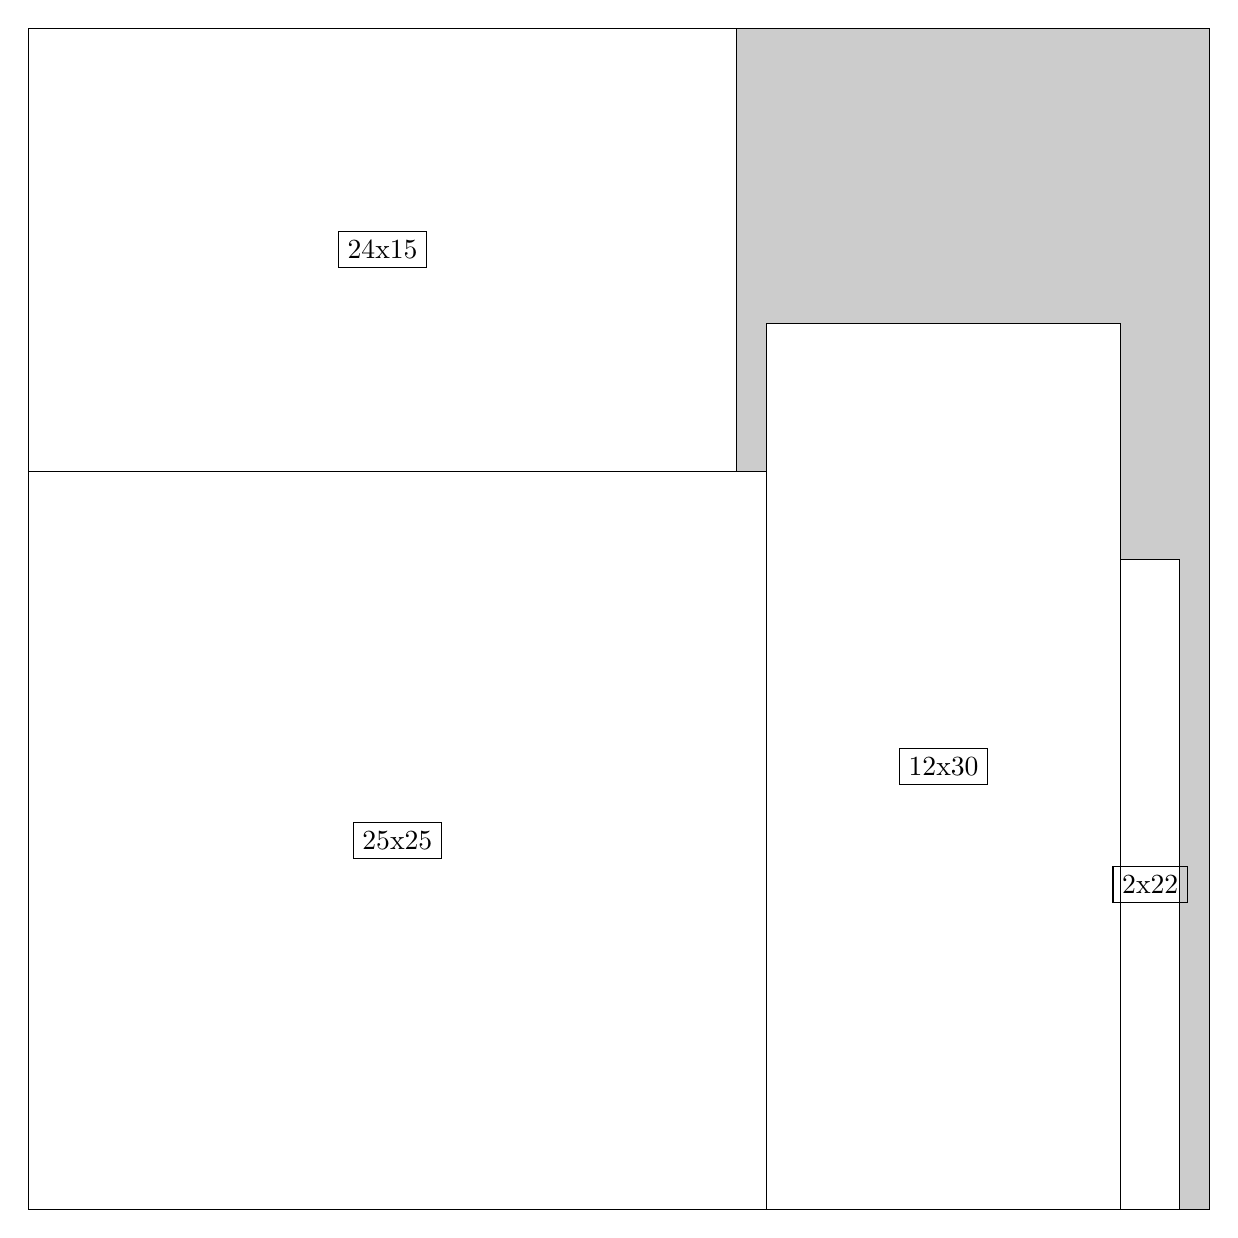
\begin{tikzpicture}[shorten >=1pt,scale=1.0,every node/.style={scale=1.0},->]
\tikzstyle{vertex}=[circle,fill=black!25,minimum size=14pt,inner sep=0pt]
\filldraw[fill=gray!40!white, draw=black] (0,0) rectangle (15.0,15.0);
\foreach \name/\x/\y/\w/\h in {25x25/0.0/0.0/9.375/9.375,24x15/0.0/9.375/9.0/5.625,12x30/9.375/0.0/4.5/11.25,2x22/13.875/0.0/0.75/8.25}
\filldraw[fill=white!40!white, draw=black] (\x,\y) rectangle node[draw] (\name) {\name} ++(\w,\h);
\end{tikzpicture}


w =25 , h =25 , x =0 , y =0 , v =625
\par
w =24 , h =15 , x =0 , y =25 , v =360
\par
w =12 , h =30 , x =25 , y =0 , v =360
\par
w =2 , h =22 , x =37 , y =0 , v =44
\par
\newpage


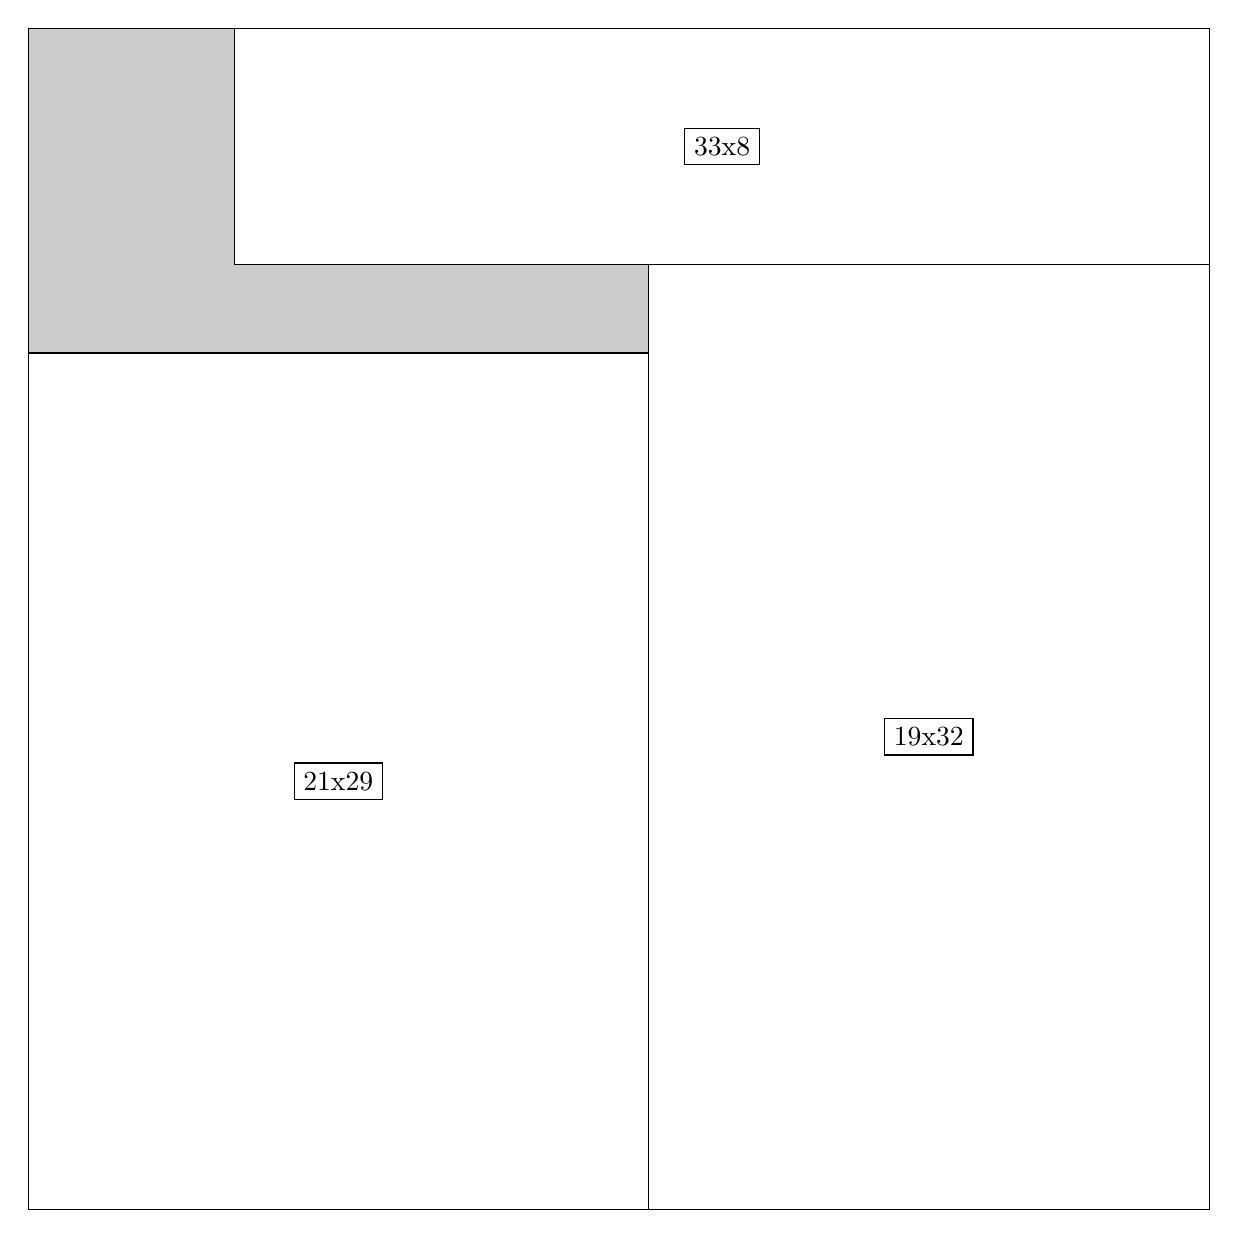
\begin{tikzpicture}[shorten >=1pt,scale=1.0,every node/.style={scale=1.0},->]
\tikzstyle{vertex}=[circle,fill=black!25,minimum size=14pt,inner sep=0pt]
\filldraw[fill=gray!40!white, draw=black] (0,0) rectangle (15.0,15.0);
\foreach \name/\x/\y/\w/\h in {21x29/0.0/0.0/7.875/10.875,19x32/7.875/0.0/7.125/12.0,33x8/2.625/12.0/12.375/3.0}
\filldraw[fill=white!40!white, draw=black] (\x,\y) rectangle node[draw] (\name) {\name} ++(\w,\h);
\end{tikzpicture}


w =21 , h =29 , x =0 , y =0 , v =609
\par
w =19 , h =32 , x =21 , y =0 , v =608
\par
w =33 , h =8 , x =7 , y =32 , v =264
\par
\newpage


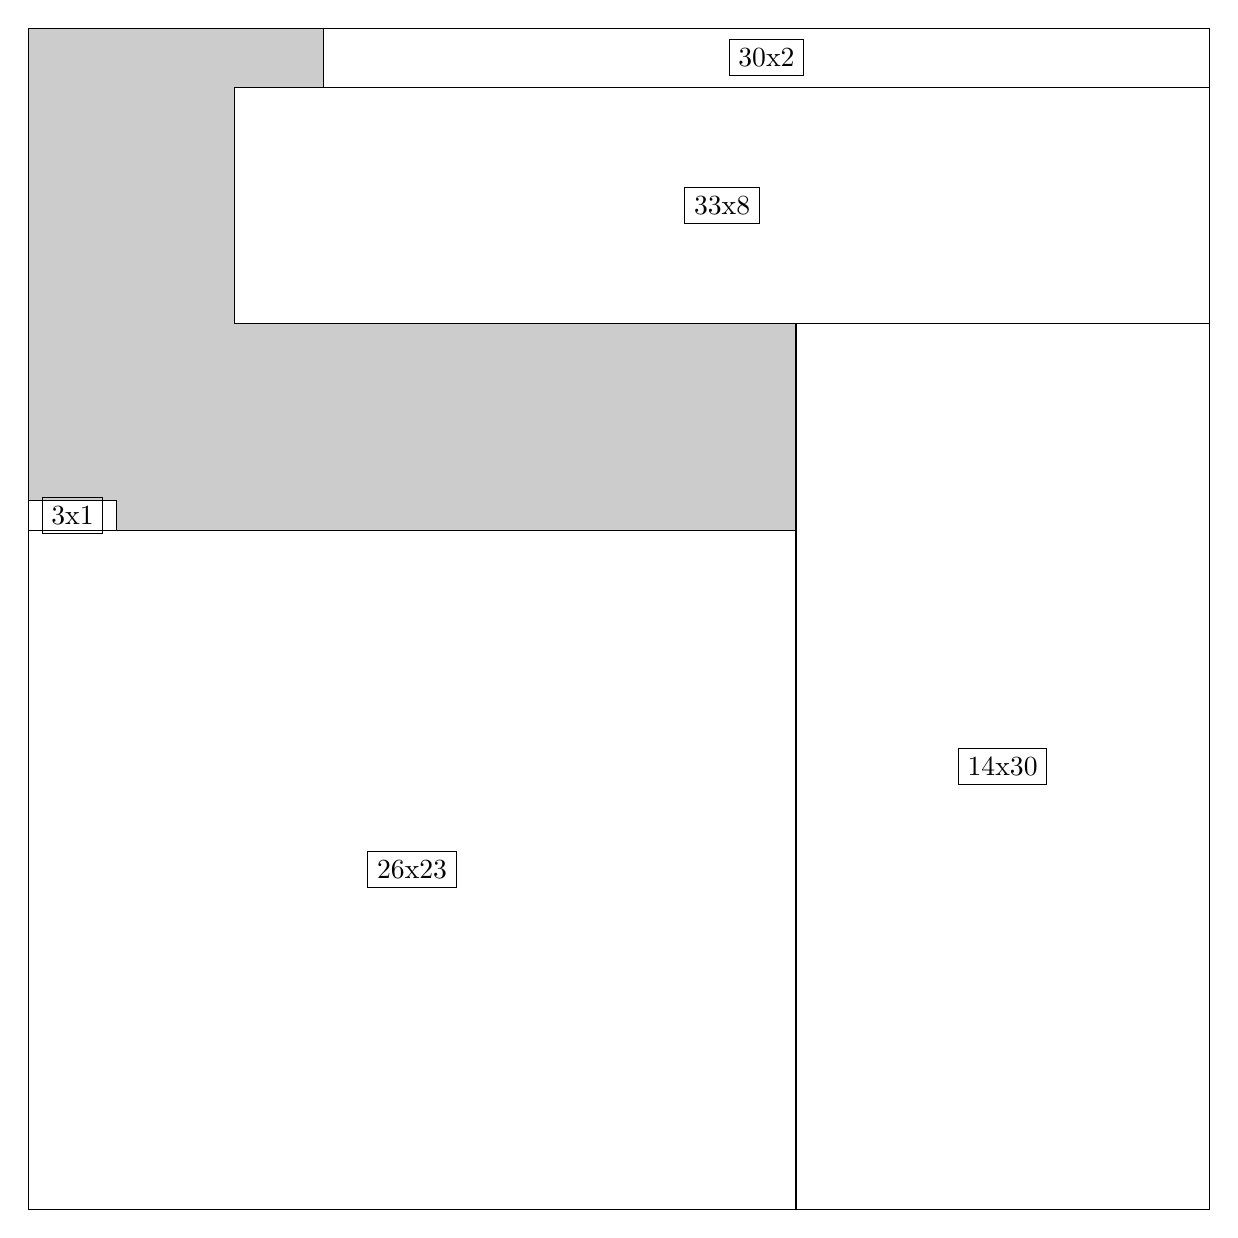
\begin{tikzpicture}[shorten >=1pt,scale=1.0,every node/.style={scale=1.0},->]
\tikzstyle{vertex}=[circle,fill=black!25,minimum size=14pt,inner sep=0pt]
\filldraw[fill=gray!40!white, draw=black] (0,0) rectangle (15.0,15.0);
\foreach \name/\x/\y/\w/\h in {26x23/0.0/0.0/9.75/8.625,14x30/9.75/0.0/5.25/11.25,33x8/2.625/11.25/12.375/3.0,30x2/3.75/14.25/11.25/0.75,3x1/0.0/8.625/1.125/0.375}
\filldraw[fill=white!40!white, draw=black] (\x,\y) rectangle node[draw] (\name) {\name} ++(\w,\h);
\end{tikzpicture}


w =26 , h =23 , x =0 , y =0 , v =598
\par
w =14 , h =30 , x =26 , y =0 , v =420
\par
w =33 , h =8 , x =7 , y =30 , v =264
\par
w =30 , h =2 , x =10 , y =38 , v =60
\par
w =3 , h =1 , x =0 , y =23 , v =3
\par
\newpage


\begin{tikzpicture}[shorten >=1pt,scale=1.0,every node/.style={scale=1.0},->]
\tikzstyle{vertex}=[circle,fill=black!25,minimum size=14pt,inner sep=0pt]
\filldraw[fill=gray!40!white, draw=black] (0,0) rectangle (15.0,15.0);
\foreach \name/\x/\y/\w/\h in {21x28/0.0/0.0/7.875/10.5,19x28/7.875/0.0/7.125/10.5,34x11/0.0/10.5/12.75/4.125,6x11/12.75/10.5/2.25/4.125,24x1/6.0/14.625/9.0/0.375}
\filldraw[fill=white!40!white, draw=black] (\x,\y) rectangle node[draw] (\name) {\name} ++(\w,\h);
\end{tikzpicture}


w =21 , h =28 , x =0 , y =0 , v =588
\par
w =19 , h =28 , x =21 , y =0 , v =532
\par
w =34 , h =11 , x =0 , y =28 , v =374
\par
w =6 , h =11 , x =34 , y =28 , v =66
\par
w =24 , h =1 , x =16 , y =39 , v =24
\par
\newpage


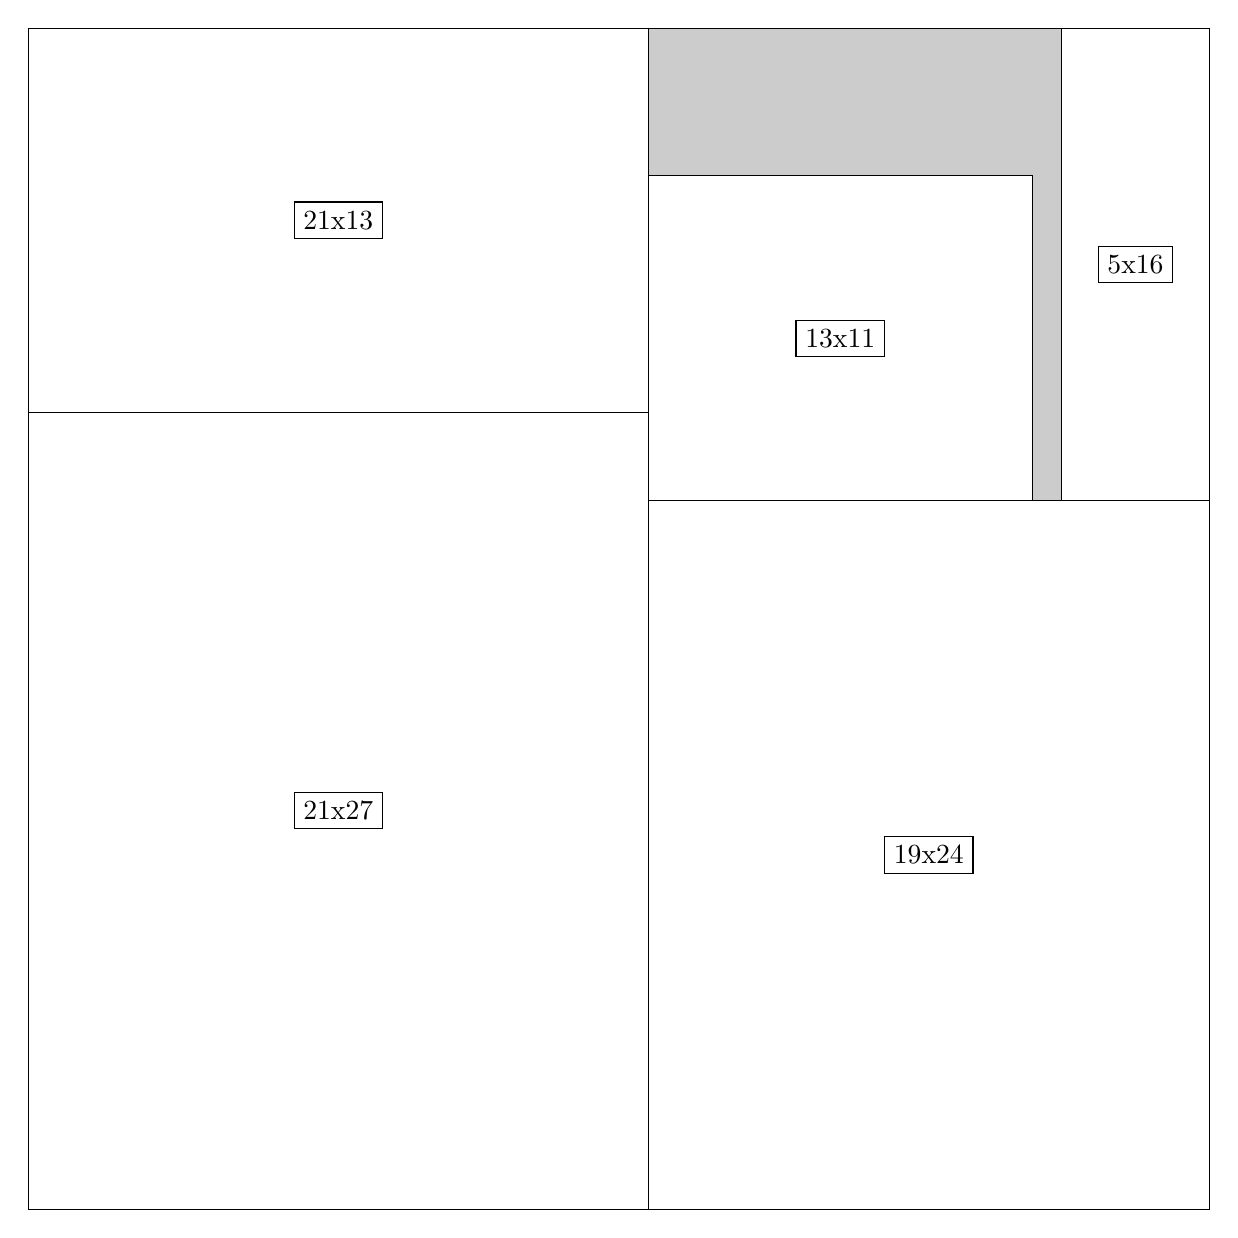
\begin{tikzpicture}[shorten >=1pt,scale=1.0,every node/.style={scale=1.0},->]
\tikzstyle{vertex}=[circle,fill=black!25,minimum size=14pt,inner sep=0pt]
\filldraw[fill=gray!40!white, draw=black] (0,0) rectangle (15.0,15.0);
\foreach \name/\x/\y/\w/\h in {21x27/0.0/0.0/7.875/10.125,19x24/7.875/0.0/7.125/9.0,21x13/0.0/10.125/7.875/4.875,13x11/7.875/9.0/4.875/4.125,5x16/13.125/9.0/1.875/6.0}
\filldraw[fill=white!40!white, draw=black] (\x,\y) rectangle node[draw] (\name) {\name} ++(\w,\h);
\end{tikzpicture}


w =21 , h =27 , x =0 , y =0 , v =567
\par
w =19 , h =24 , x =21 , y =0 , v =456
\par
w =21 , h =13 , x =0 , y =27 , v =273
\par
w =13 , h =11 , x =21 , y =24 , v =143
\par
w =5 , h =16 , x =35 , y =24 , v =80
\par
\newpage


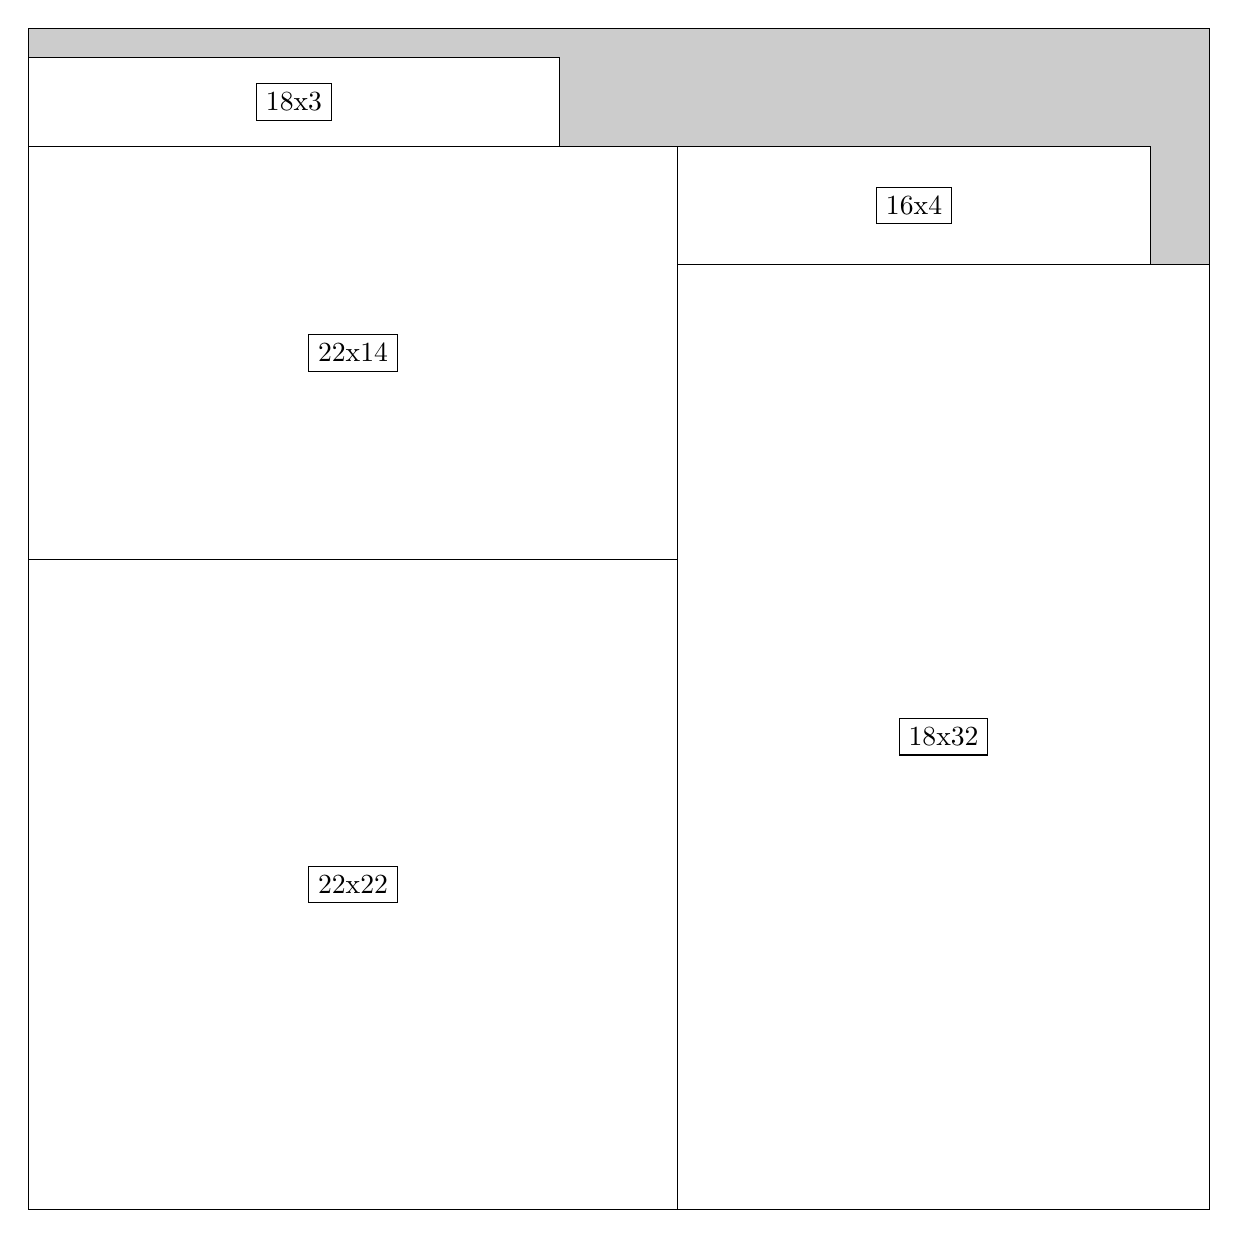
\begin{tikzpicture}[shorten >=1pt,scale=1.0,every node/.style={scale=1.0},->]
\tikzstyle{vertex}=[circle,fill=black!25,minimum size=14pt,inner sep=0pt]
\filldraw[fill=gray!40!white, draw=black] (0,0) rectangle (15.0,15.0);
\foreach \name/\x/\y/\w/\h in {18x32/8.25/0.0/6.75/12.0,22x22/0.0/0.0/8.25/8.25,22x14/0.0/8.25/8.25/5.25,16x4/8.25/12.0/6.0/1.5,18x3/0.0/13.5/6.75/1.125}
\filldraw[fill=white!40!white, draw=black] (\x,\y) rectangle node[draw] (\name) {\name} ++(\w,\h);
\end{tikzpicture}


w =18 , h =32 , x =22 , y =0 , v =576
\par
w =22 , h =22 , x =0 , y =0 , v =484
\par
w =22 , h =14 , x =0 , y =22 , v =308
\par
w =16 , h =4 , x =22 , y =32 , v =64
\par
w =18 , h =3 , x =0 , y =36 , v =54
\par
\newpage


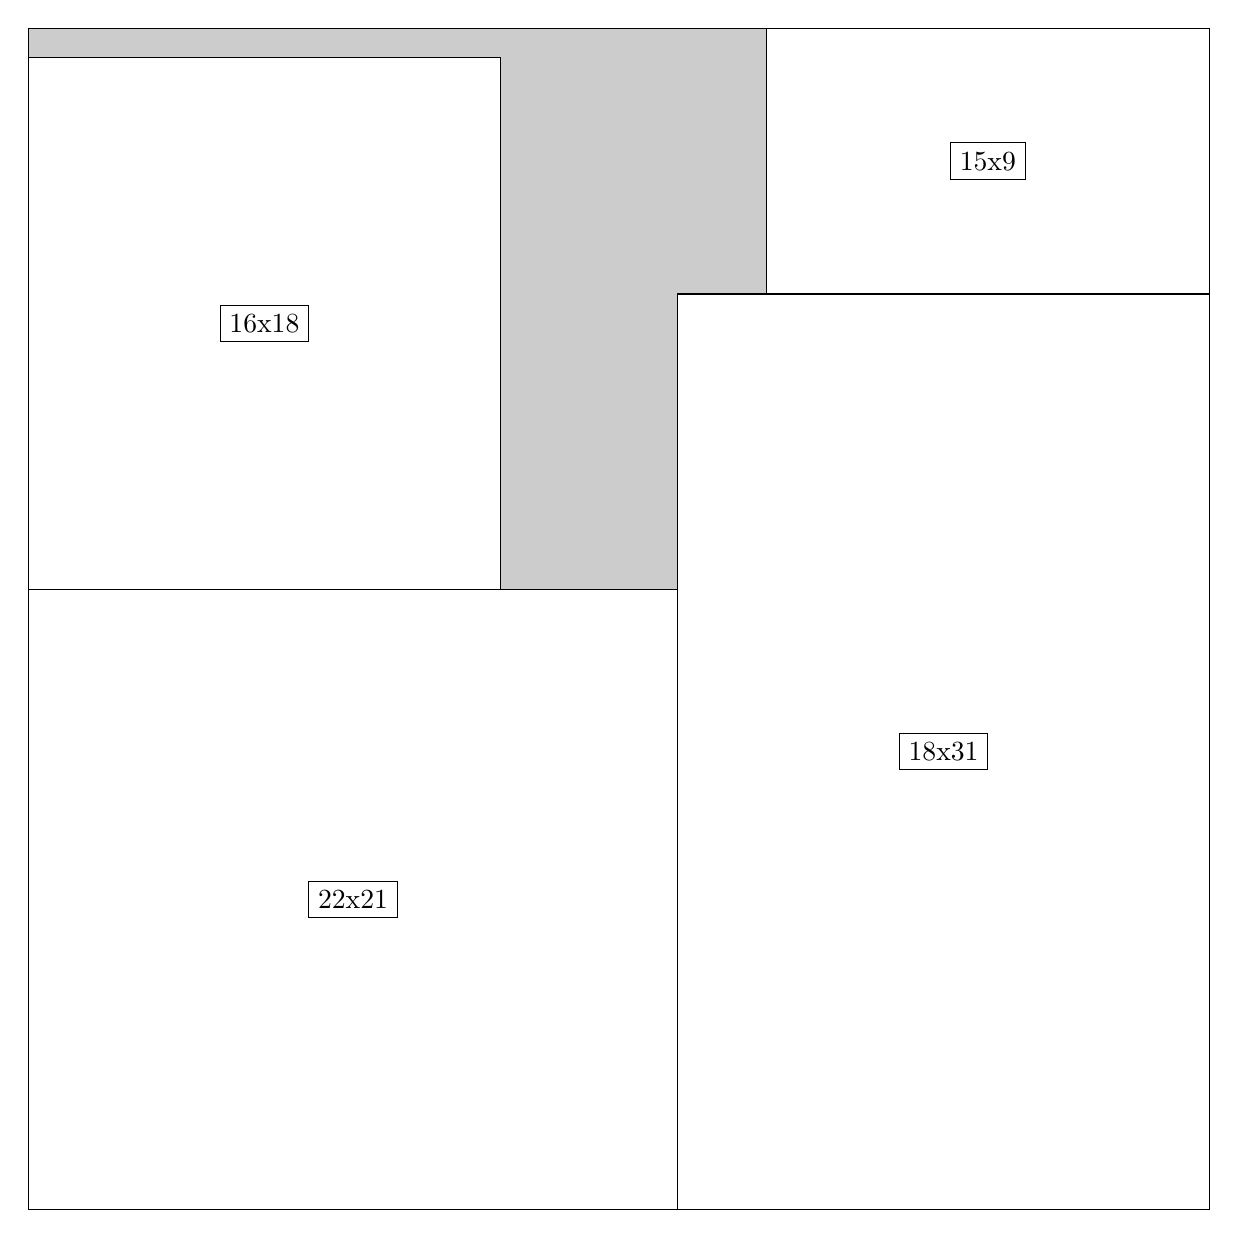
\begin{tikzpicture}[shorten >=1pt,scale=1.0,every node/.style={scale=1.0},->]
\tikzstyle{vertex}=[circle,fill=black!25,minimum size=14pt,inner sep=0pt]
\filldraw[fill=gray!40!white, draw=black] (0,0) rectangle (15.0,15.0);
\foreach \name/\x/\y/\w/\h in {18x31/8.25/0.0/6.75/11.625,22x21/0.0/0.0/8.25/7.875,16x18/0.0/7.875/6.0/6.75,15x9/9.375/11.625/5.625/3.375}
\filldraw[fill=white!40!white, draw=black] (\x,\y) rectangle node[draw] (\name) {\name} ++(\w,\h);
\end{tikzpicture}


w =18 , h =31 , x =22 , y =0 , v =558
\par
w =22 , h =21 , x =0 , y =0 , v =462
\par
w =16 , h =18 , x =0 , y =21 , v =288
\par
w =15 , h =9 , x =25 , y =31 , v =135
\par
\newpage


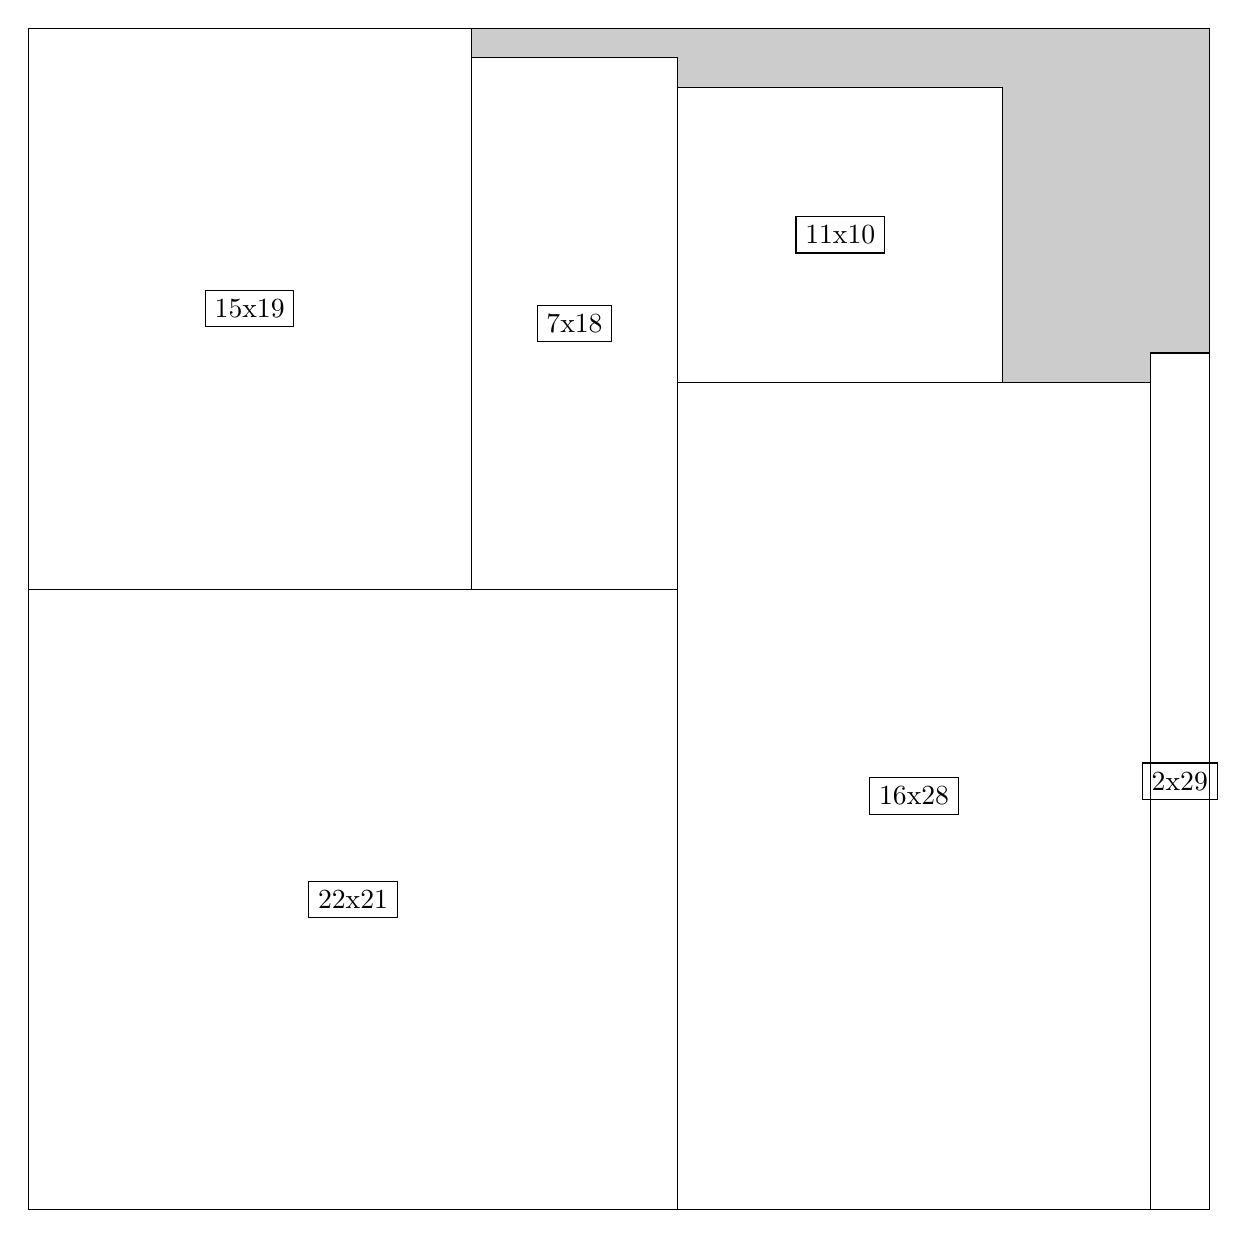
\begin{tikzpicture}[shorten >=1pt,scale=1.0,every node/.style={scale=1.0},->]
\tikzstyle{vertex}=[circle,fill=black!25,minimum size=14pt,inner sep=0pt]
\filldraw[fill=gray!40!white, draw=black] (0,0) rectangle (15.0,15.0);
\foreach \name/\x/\y/\w/\h in {22x21/0.0/0.0/8.25/7.875,16x28/8.25/0.0/6.0/10.5,15x19/0.0/7.875/5.625/7.125,7x18/5.625/7.875/2.625/6.75,11x10/8.25/10.5/4.125/3.75,2x29/14.25/0.0/0.75/10.875}
\filldraw[fill=white!40!white, draw=black] (\x,\y) rectangle node[draw] (\name) {\name} ++(\w,\h);
\end{tikzpicture}


w =22 , h =21 , x =0 , y =0 , v =462
\par
w =16 , h =28 , x =22 , y =0 , v =448
\par
w =15 , h =19 , x =0 , y =21 , v =285
\par
w =7 , h =18 , x =15 , y =21 , v =126
\par
w =11 , h =10 , x =22 , y =28 , v =110
\par
w =2 , h =29 , x =38 , y =0 , v =58
\par
\newpage


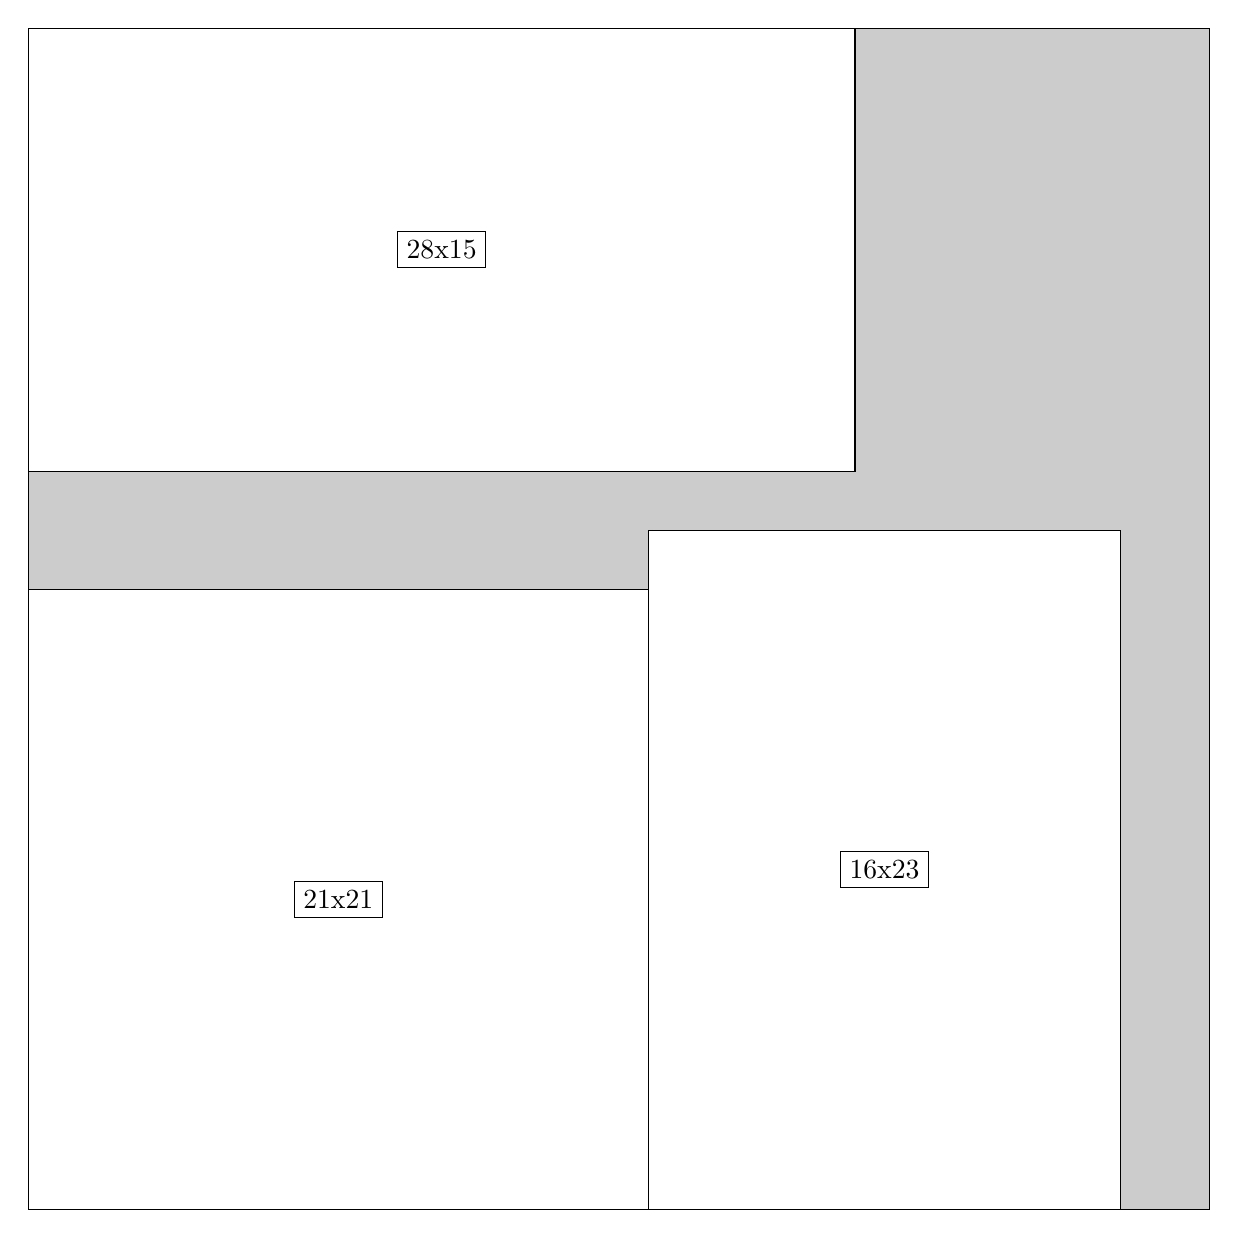
\begin{tikzpicture}[shorten >=1pt,scale=1.0,every node/.style={scale=1.0},->]
\tikzstyle{vertex}=[circle,fill=black!25,minimum size=14pt,inner sep=0pt]
\filldraw[fill=gray!40!white, draw=black] (0,0) rectangle (15.0,15.0);
\foreach \name/\x/\y/\w/\h in {21x21/0.0/0.0/7.875/7.875,28x15/0.0/9.375/10.5/5.625,16x23/7.875/0.0/6.0/8.625}
\filldraw[fill=white!40!white, draw=black] (\x,\y) rectangle node[draw] (\name) {\name} ++(\w,\h);
\end{tikzpicture}


w =21 , h =21 , x =0 , y =0 , v =441
\par
w =28 , h =15 , x =0 , y =25 , v =420
\par
w =16 , h =23 , x =21 , y =0 , v =368
\par
\newpage


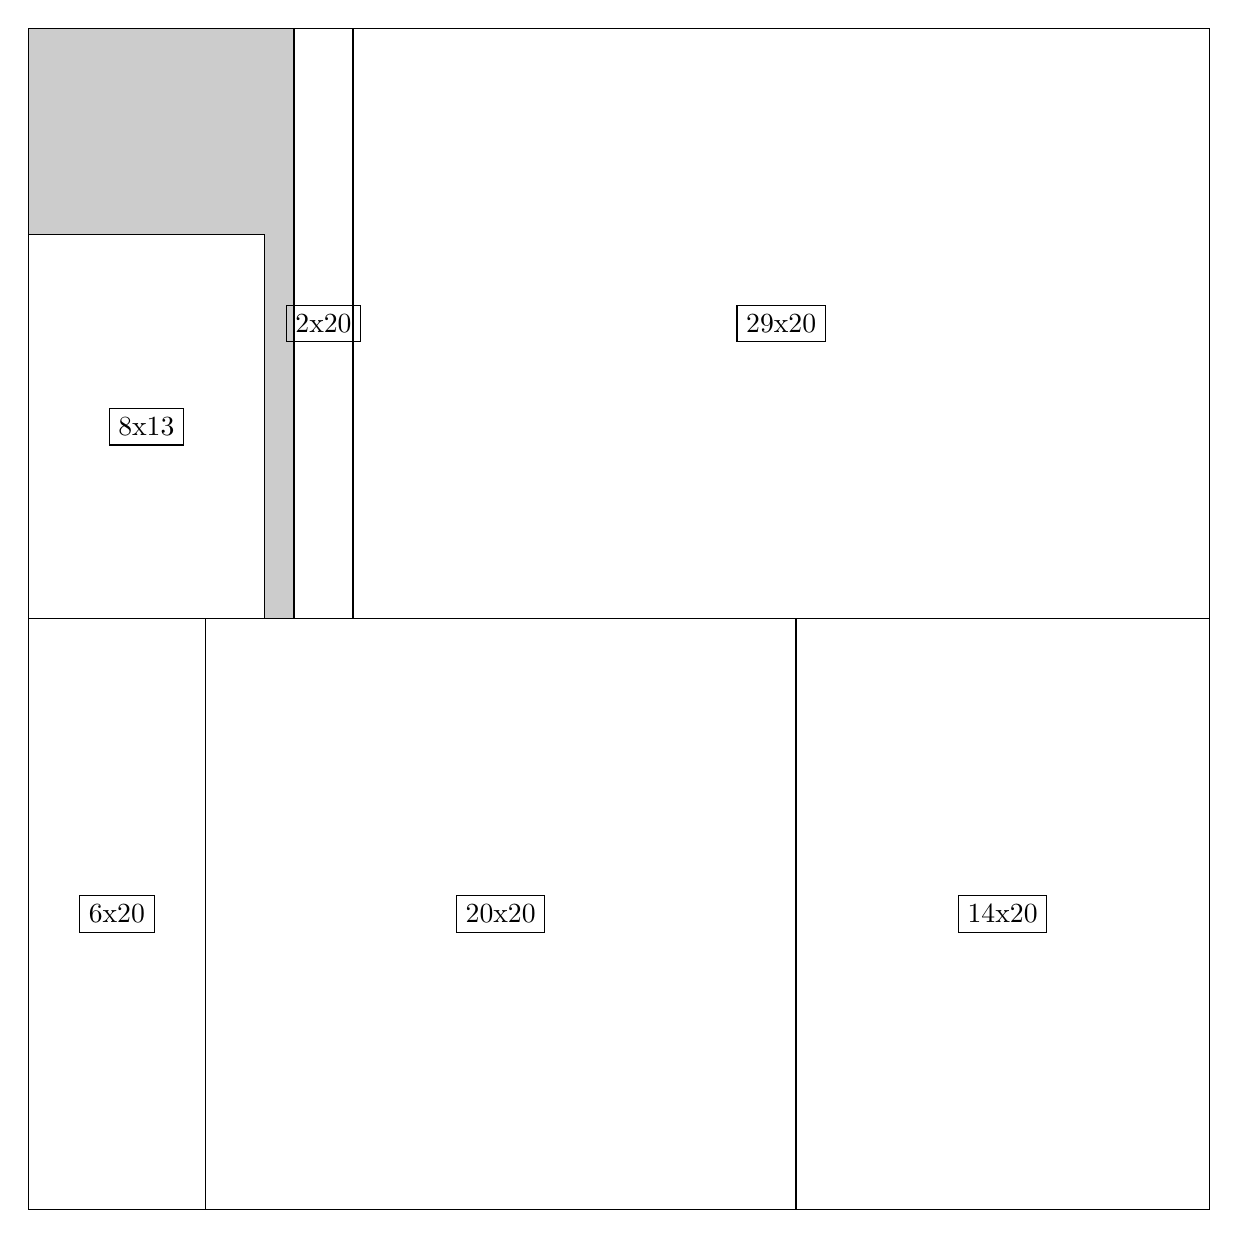
\begin{tikzpicture}[shorten >=1pt,scale=1.0,every node/.style={scale=1.0},->]
\tikzstyle{vertex}=[circle,fill=black!25,minimum size=14pt,inner sep=0pt]
\filldraw[fill=gray!40!white, draw=black] (0,0) rectangle (15.0,15.0);
\foreach \name/\x/\y/\w/\h in {6x20/0.0/0.0/2.25/7.5,20x20/2.25/0.0/7.5/7.5,14x20/9.75/0.0/5.25/7.5,29x20/4.125/7.5/10.875/7.5,8x13/0.0/7.5/3.0/4.875,2x20/3.375/7.5/0.75/7.5}
\filldraw[fill=white!40!white, draw=black] (\x,\y) rectangle node[draw] (\name) {\name} ++(\w,\h);
\end{tikzpicture}


w =6 , h =20 , x =0 , y =0 , v =120
\par
w =20 , h =20 , x =6 , y =0 , v =400
\par
w =14 , h =20 , x =26 , y =0 , v =280
\par
w =29 , h =20 , x =11 , y =20 , v =580
\par
w =8 , h =13 , x =0 , y =20 , v =104
\par
w =2 , h =20 , x =9 , y =20 , v =40
\par
\newpage


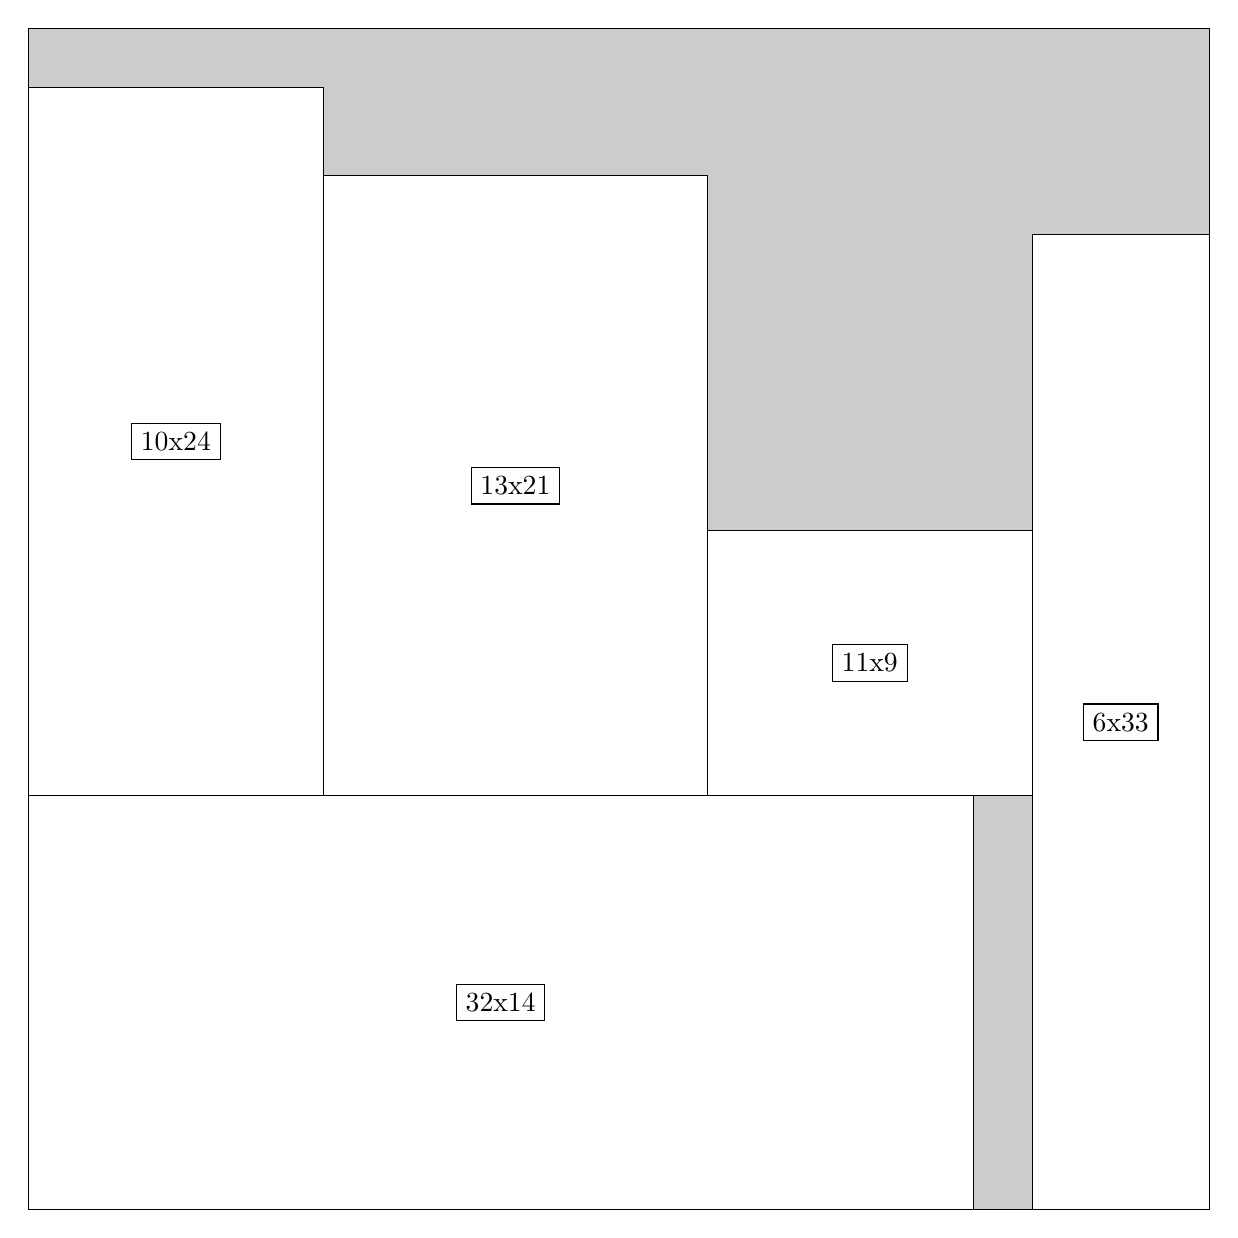
\begin{tikzpicture}[shorten >=1pt,scale=1.0,every node/.style={scale=1.0},->]
\tikzstyle{vertex}=[circle,fill=black!25,minimum size=14pt,inner sep=0pt]
\filldraw[fill=gray!40!white, draw=black] (0,0) rectangle (15.0,15.0);
\foreach \name/\x/\y/\w/\h in {32x14/0.0/0.0/12.0/5.25,13x21/3.75/5.25/4.875/7.875,10x24/0.0/5.25/3.75/9.0,6x33/12.75/0.0/2.25/12.375,11x9/8.625/5.25/4.125/3.375}
\filldraw[fill=white!40!white, draw=black] (\x,\y) rectangle node[draw] (\name) {\name} ++(\w,\h);
\end{tikzpicture}


w =32 , h =14 , x =0 , y =0 , v =448
\par
w =13 , h =21 , x =10 , y =14 , v =273
\par
w =10 , h =24 , x =0 , y =14 , v =240
\par
w =6 , h =33 , x =34 , y =0 , v =198
\par
w =11 , h =9 , x =23 , y =14 , v =99
\par
\newpage


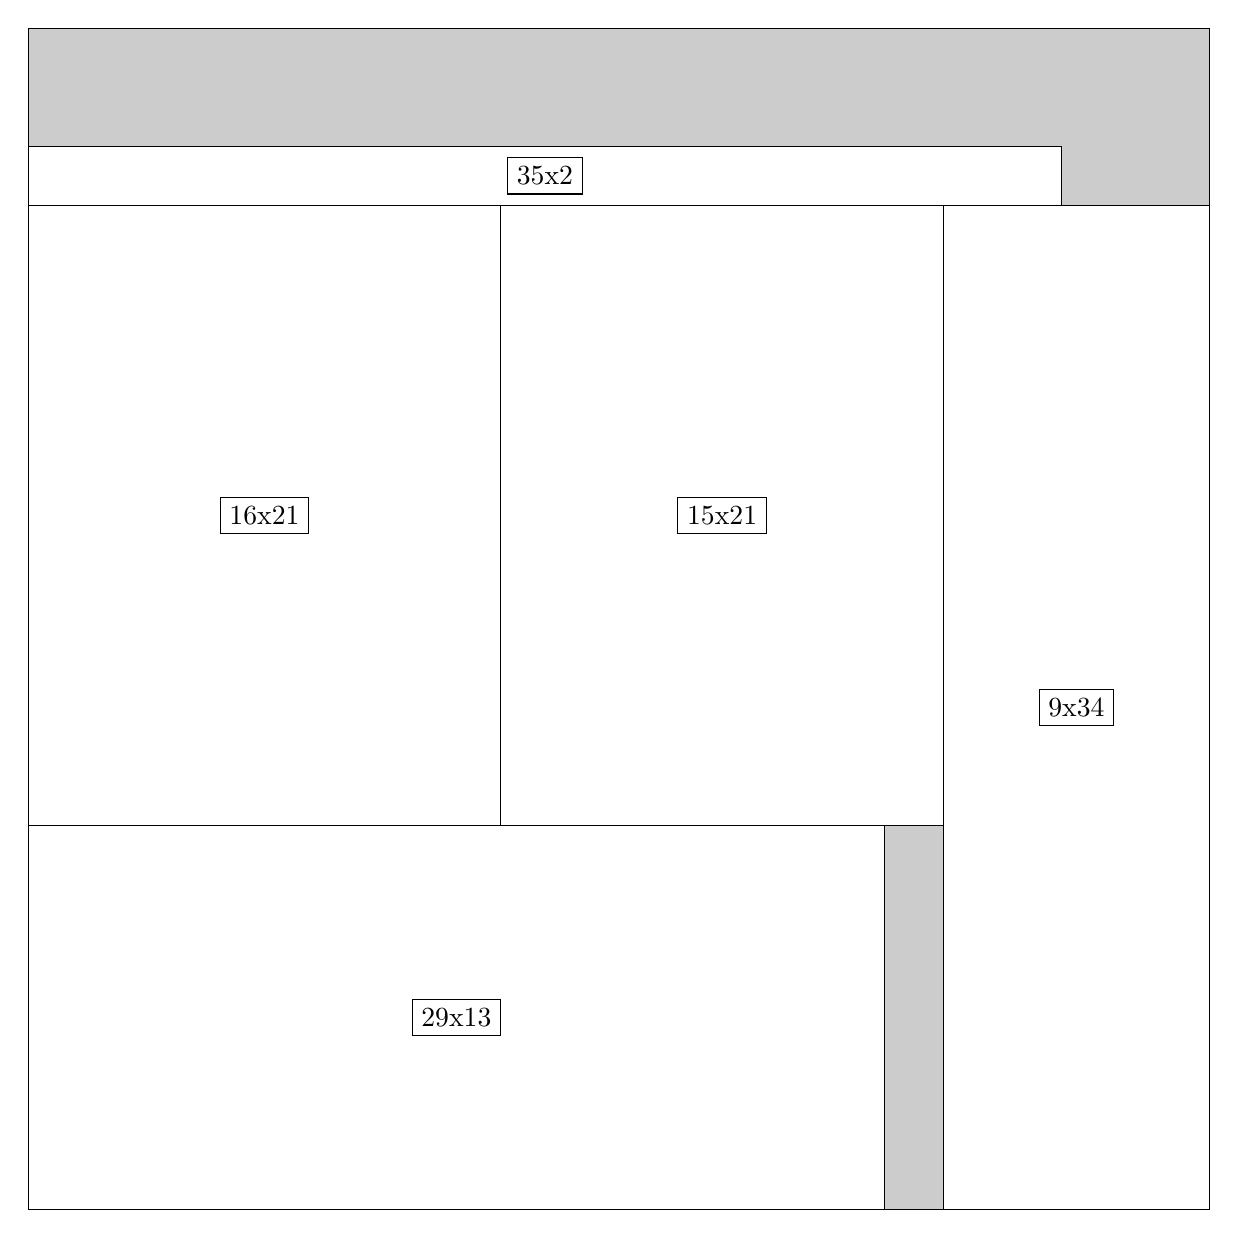
\begin{tikzpicture}[shorten >=1pt,scale=1.0,every node/.style={scale=1.0},->]
\tikzstyle{vertex}=[circle,fill=black!25,minimum size=14pt,inner sep=0pt]
\filldraw[fill=gray!40!white, draw=black] (0,0) rectangle (15.0,15.0);
\foreach \name/\x/\y/\w/\h in {29x13/0.0/0.0/10.875/4.875,16x21/0.0/4.875/6.0/7.875,15x21/6.0/4.875/5.625/7.875,9x34/11.625/0.0/3.375/12.75,35x2/0.0/12.75/13.125/0.75}
\filldraw[fill=white!40!white, draw=black] (\x,\y) rectangle node[draw] (\name) {\name} ++(\w,\h);
\end{tikzpicture}


w =29 , h =13 , x =0 , y =0 , v =377
\par
w =16 , h =21 , x =0 , y =13 , v =336
\par
w =15 , h =21 , x =16 , y =13 , v =315
\par
w =9 , h =34 , x =31 , y =0 , v =306
\par
w =35 , h =2 , x =0 , y =34 , v =70
\par
\newpage


\end{document}